\documentclass[fleqn,11pt]{report}
\usepackage{amsmath,amssymb,esint}
\usepackage{amsthm,fixmath}
\usepackage[english]{babel}
\usepackage[a4paper,total={170mm,257mm},]{geometry}
\usepackage{epsfig}
\usepackage[format=hang,justification=centering]{subfig}
\usepackage{multirow}
\usepackage[square,comma,numbers,sort&compress]{natbib}
\usepackage{graphics}
\usepackage{graphicx}
\usepackage{hyperref}
\usepackage{float}
\usepackage{enumitem}
\usepackage{color}
\usepackage[x11names]{xcolor}
\usepackage{setspace}
\usepackage{listings}
\usepackage[UKenglish]{isodate}
\usepackage{fancybox}
\usepackage{fancyheadings,tabularx}
\usepackage{longtable}
\usepackage{ulem}
\usepackage{paralist}
\usepackage{placeins}
\usepackage{tabto}

\pagestyle{fancyplain}  

\definecolor{C_Green}{rgb}{0,0.6,0}
\definecolor{C_Gray}{rgb}{0.5,0.5,0.5}
\definecolor{G_Purple}{rgb}{0.58,0,0.82}
\definecolor{C_Background}{rgb}{0.95,0.95,0.92}

\lstdefinestyle{CStyle}{
    backgroundcolor=\color{C_Background},   
    commentstyle=\ttfamily\color{C_Green},
    keywordstyle=\ttfamily\color{magenta},
    numberstyle=\ttfamily\tiny\color{C_Gray},
    stringstyle=\ttfamily\color{G_Purple},
    basicstyle=\ttfamily\footnotesize,
    breakatwhitespace=false,         
    breaklines=true,                 
    captionpos=b,                    
    keepspaces=true,                 
    numbers=left,                    
    numbersep=5pt,                  
    showspaces=false,                
    showstringspaces=false,
    showtabs=false,                  
    tabsize=2,
    language=C
}

\graphicspath{{figures/}} 

\usepackage[intoc]{nomencl}
\setcounter{secnumdepth}{3}
\setcounter{tocdepth}{2}
\setcounter{topnumber}{4}
\setcounter{totalnumber}{5}
\renewcommand{\topfraction}{1}
\renewcommand{\bottomfraction}{1}
\renewcommand{\textfraction}{0.01}
\newfloat{Program}{h}{lop}[chapter]
\newcommand{\HRule}{\rule{\linewidth}{0.5mm}}
\newcommand{\thedate}{\today}
\cleanlookdateon

\pagestyle{fancy}
\renewcommand{\headrulewidth}{0pt}
\renewcommand{\footrulewidth}{0.4pt}
\fancyhf{}
\lfoot{https://github.com/polycfd/Wave-DNA}
\cfoot{\thepage}
\rfoot{\thedate}

\fancypagestyle{plain}{%
  \fancyhf{}%
  \lfoot{https://github.com/polycfd/apecss}
  \cfoot{\thepage}
  \rfoot{\thedate}
  \renewcommand{\headrulewidth}{0pt}% Line at the header invisible
  \renewcommand{\footrulewidth}{0.4pt}% Line at the footer visible
}

\hypersetup{colorlinks = true, urlcolor = RoyalBlue3, linkcolor = RoyalBlue3, citecolor = RoyalBlue3}

\setlength{\parindent}{0cm}
\setlength{\parskip}{0.7em}
\setlength{\itemsep}{1pt}
\renewcommand{\em}{\it}
%%%%%%%%%%%%%%%%%%%%%%%%%%%%%%%%%%%%%%%%%%%%%%%%%%%%%%%%%%%%%%%%
\begin{document}
% Title Page
\begin{titlepage}
\begin{center}
% Upper part of the page
\null \vfill
% Title
\HRule \\[0.4cm]
{\huge Wave-DNA}\\[0.05cm] {\large (Wave-Doppler-shifts in nonlinear acoustics)}\\[0.1cm]
\HRule \\[2cm]

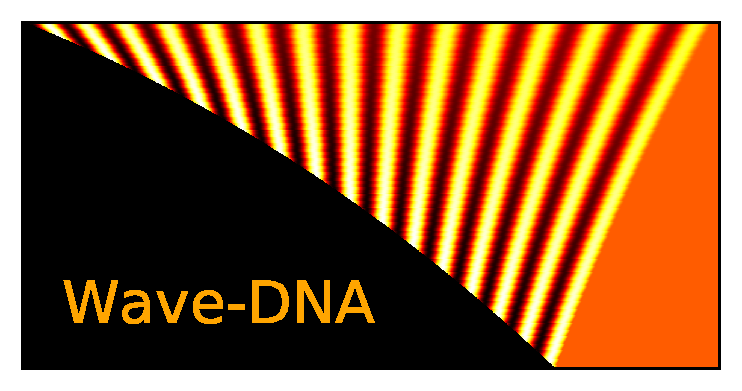
\includegraphics[width=0.5\textwidth]{{figures/rt_cover}.pdf}

\vspace{5cm}
S\"oren Schenke\\
Fabian Sewerin\\
Berend van Wachem\\
Fabian Denner
\vfill

\thedate

\end{center}
\end{titlepage}

{\hypersetup{linkcolor=black}
\tableofcontents 
}

\chapter{About Wave-DNA}
\label{chap:About Wave-DNA}

{\tt Wave-DNA} is a simulation tool for one-dimensional and spherically-symmetric nonlinear acoustic waves in transient and spatially variable background flow fields. The motion of the background medium is accounted for by considering a convective form of the lossless Kuznetsov wave equation \citep{Schenke_et_al_2023_JASA}, derived from first principles based on perturbations of the continuity equation and the transient Bernoulli equation. The background flow field in which the acoustic waves propagate is treated as an input to the wave solver. In principle, the background flow field my be obtained from analytical considerations, numerical simulations, or experimental measurements. The tool recommends itself for the fundamental study of nonlinear Doppler phenomena in acoustic wave propagation.

The moving boundary may represent a moving wave emitter or scatterer, and it may move relative to the fluid or displace the surrounding fluid. This allows the user to study nonlinear Doppler effects associated with moving wave emitters/scatterers and/or non-uniform background flow fields. The motion of the domain boundary is conveniently taken into account by a generic coordinate transformation of the governing wave equation, where the transformed wave equation is solved in a fixed computational domain. This technique enables accurate numerical solutions of the combined wave-flow problem without the necessity to interpolate data between the moving grid points in the physical domain. The numerical technique is based on explicit finite differences, and it is equipped with a predictor-corrector method to counteract the onset and growth of dispersive numerical noise in the cases of broad frequency bands or shock formation \citep{Schenke_et_al_2022}. Furthermore, absorbing boundary conditions can be imposed in order to let the acoustic waves pass the domain boundaries without reflection.

A particularly well-suited example to demonstrate the capability of the simulation framework is the so-called acoustic black/white hole analogue as presented in \citep{Schenke_et_al_2022_PoF, Schenke_et_al_2023_JASA}. The present documentation provides detailed instructions on how to conduct acoustic black and white hole simulations using {\tt Wave-DNA}, as well as other examples to demonstrate the capabilities and functionalities of the tool.

The {\tt Wave-DNA} repository is located at \href{https://github.com/polycfd/Wave-DNA}{\texttt{https://github.com/polycfd/Wave-DNA}}, is under the copyright of its developers and made available as open-source software under the terms of the \href{https://opensource.org/license/mit/}{MIT License}. Details about the theory and numerical methods of {\tt Wave-DNA}, as well as examples of its scientific applications, can be found in these papers: \citep{Schenke_et_al_2022, Schenke_et_al_2022_PoF, Schenke_et_al_2023_JASA}.
The development of {\tt Wave-DNA} has directly benefitted from research funding provided by the Deutsche Forschungsgemeinschaft (DFG, German Research Foundation), grant number 441063377.



\chapter{Using Wave-DNA}
\label{chap:Using Wave-DNA}



\section{Installation}
\label{sec:Installation}

It is convenient to compile the source code in a build directory separate from the source directory by executing the {\tt cleanbuild\_release.sh} script to compile in optimized release mode, or by excecuting the {\tt cleanbuild\_debug.sh} script to compile in debug mode. The program runs significantly faster in release mode.

By running the build scripts ({\tt cleanbuild\_release.sh} or {\tt cleanbuild\_debug.sh}), all files in the build directory that were previously generated by {\tt cmake} are removed. Subsequently, a {\tt cmake} run is performed on the {\tt CMakeLists.txt} file. In the {\tt CMakeLists.txt} file, the {\tt gcc} compiler must be set as {\tt CMAKE\_C\_COMPILER}, providing the path to the {\tt gcc} executable. For instance:
\\[8pt]
{\tt set(CMAKE\_C\_COMPILER /usr/bin/gcc)}
\\[8pt]
Furthermore, the environmental variable  {\tt \${mylibdirs}} must be set in {\tt CMakeLists.txt}. For instance:
\\[8pt]
{\tt set(mylibdirs \${mylibdirs} /usr/lib64/)}
\\[8pt]
Finally, the {\tt Wave-DNA} source directory must be specified. This is done by either directly setting the path to the source directory as
\\[8pt]
{\tt FILE (GLOB\_RECURSE MYFILES ABSOLUTE  /path/to/wavedna/src/*.c)}
\\[8pt]
or by setting:
\\[8pt]
{\tt FILE (GLOB\_RECURSE MYFILES ABSOLUTE  \$ENV\{WaveDNA\_DIR\}/src/*.c)}
\\[8pt]
The latter option requires to set the environmental variable {\tt \$WaveDNA\_DIR} to {\tt /path/to/wavedna} in the configuration file of the {\tt Unix} shell, as for instance {\tt /path/to/home/.bashrc}. With the default settings in the provided {\tt CMakeLists.txt} file, the executable {\tt WaveDNA} is created in the build directory upon successful compilation. See the following lines in {\tt CMakeLists.txt}:
\\[8pt]
{\tt add\_executable(WaveDNA \$\{MYFILES\})} \\
{\tt target\_link\_libraries(WaveDNA \$\{mylibs\})}
\\[8pt]


\section{Running a simulation}
\label{sec:Running a simulation}

The simulation case directory needs to have an options file, called {\tt run.DNA} by default, which contains the user options\footnote{If the file is empty, a default run is performed based on the default options as indicated in Section \ref{sec:Default settings} (also see {\tt src/io/iodefaultoptions.c})}, and a {\tt results} directory is generated upon executing {\tt Wave-DNA}, in which the the output files are written. The simulation is run in the case directory by executing the following command:
\\[8pt]
{\tt /path/to/some/arbitrary/build/directory/WaveDNA}
\\[8pt]
The options file may also take another name different from {\tt run.DNA}. In that case, the simulation must be executed with the following command line option:
\\[8pt]
{\tt /path/to/some/arbitrary/build/directory/WaveDNA -options optionsFileName}
\\[8pt]


\section{Run options and fluid properties}
\label{sec:Run options and fluid properties}

The basic run options and fluid properties are set in the sections {\tt RUNOPTIONS} and {\tt FLUID}, respectively. Next to the background density and speed of sound, $\rho_0$ and $c_0$, respectively, one can specify the nonlinearity coefficient $\beta$ to admit cumulative nonlinearities. Independent of this option, one can further indicate, whether local nonlinearties (a non-zero Lagrangian density $\mathcal{L}$) are taken into account. By this means, one can effectively solve
\begin{compactitem}
\item the linear wave equation ($\beta = 0$, $\mathcal{L}=0$),
\item the lossless Westervelt equation ($\beta \neq 0$, $\mathcal{L}=0$) \citep{Schenke_et_al_2022},
\item or the lossless Kuznetsov equation ($\beta \neq 0$, $\mathcal{L}\neq 0$) \citep{Schenke_et_al_2023_JASA}.
\end{compactitem}
The following table provides a detailed overview of the run and fluid property options.

\noindent
\begin{longtable}{p{0.4\textwidth} p{0.55\textwidth}}
\textbf{Command} & \textbf{Description}
\vspace{1mm} \\
\hline Section {\tt RUNOPTIONS} &\\ \hline
{\tt TimeStart <float>} & Physical start time of the simulation. \\
{\tt TimeEnd <float>} & Physical end time of the simulation. \\{\tt WriteFrequency <float>} & Number of time steps between successive write to disc occurrences. This determines the time instances at which the field data is written to disc (fields.dat). The data recorded at sample points is stored in buffer and written to disc (probes.dat) at this occasion as well. \\
{\tt SamplePoints <int> <float> ...} & Number of sample points ({\tt <int>}) followed by the coordinates ({\tt <float>}) of the sample points. The nearest neighbour grid points to the target locations and their IDs is identified and the sample is taken at those grid points throughout the entire simulation. This means that the probe is moving with the grid. If the indicated number of sample points is larger than zero and does not match the number of given points, the simulation aborts with the error message "{\tt An unknown option ...}". \\
\\
\hline Section {\tt FLUID} &\\ \hline
{\tt SoundSpeed <float>} & Background speed of sound $c_0$ of the fluid. \\
{\tt Density <float>} & Background density $\rho_0$ of the fluid. \\
{\tt FluidNonLinearity <float>} & Nonlinearity coefficient $\beta$ of the fluid. \\
{\tt LocalNonlinearity <string>} & If set to {\tt True}, the second-order acoustic terms giving rise to local nonlinear wave propagation are active. The option {\tt False} (default) in combination with a non-zero value for $\beta$ effectively means that the Westervelt equation is solved. \\
 \hline
\end{longtable} \vspace{1em}


\section{Wave excitation}
\label{sec:Wave excitation}

Several options are available to excite an acoustic pressure wave at a specific emission node. The present modeling framework is particularly designed to solve boundary value problems, where the domain boundaries act as wave-emitting boundaries. Before explaining the the different types of excitation functions, there some important remarks:

\begin{compactitem}
\item The moving boundary is always associated with the grid node 0, regardless of whether its coordinate $R\left(t\right)$ takes a larger or smaller value than the coordinate $R_{\mathrm{stat}}$ of the fixed boundary. This means that the grid node $N_{\mathrm{points}}-1$ is always associated with the fixed boundary $R_{\mathrm{stat}}$.
\item Only one single excitation node can be specified in the present version.
\item The user is free to specify any node between $0$ and $N_{\mathrm{points}}-1$. However, as the present modeling framework is specifically designed to solve boundary value problems, the source pressure is not a volumetric source.
\item The emission of the acoustic pressure as specified by the excitation function is always strictly enforced as per the applied boundary condition, regardless of whether the wave-emitting boundary is in relative motion to the background medium or not. Consequently, the effect of convective amplification/attenuation, which relies on the Doppler-factor of the relative motion between emitter and background medium \citep{Ostashev_et_al_2005}, must be taken into account in the specification of the emitted acoustic pressure amplitude.
\end{compactitem}

The sinusoidal excitation function for the acoustic pressure $p_1$ at the emission node is given by
\begin{equation}
\left.p_1\left(t\right)\right|_{\mathrm{emission\:node}} = G\left(t\right)\Delta p_{\mathrm{a}}\left[\sin\left(2\pi f_{\mathrm{a}}t - \Delta \varphi\right)\right]^n,
\label{eq:ExcitationSine}
\end{equation}
where $\Delta p_{\mathrm{a}}$, $f_{\mathrm{a}}$, and $\Delta \phi$ are the emitted acoustic pressure amplitude, the excitation frequency and a fixed phase shift, respectively. The sine function can be raised to a power $n$, to admit nonlinearities in the excitation signal. The factor $G\left(t\right)$ is a Gauss function given by
\begin{equation}
\left.G\left(t\right)\right|_{\mathrm{emission\:node}} = q^{4\left(f_{\mathrm{a}}t - N + 1/2\right)^2},
\label{eq:GaussEnvelope}
\end{equation}
which has a peak value of unity and where $q$ is a shape coefficient that specifies the width of the Gaussian. Eq. \eqref{eq:GaussEnvelope} can be used in conjunction with Eq. \eqref{eq:ExcitationSine} to define a Gauss-enveloped sinusoidal excitation signal, where Gaussian peaks at the center of the $N^{\textnormal{th}}$ period. Alternatively, it can be used to emit a Gaussian pulse $\Delta p_{\mathrm{a}}G\left(t\right)$, where $f_{\mathrm{a}}$ and $N$ as well $\Delta _{\mathrm{a}}$ must be specified to indicate the center time and the amplitude of the pulse, respectively. The parameters of Eqs. \eqref{eq:ExcitationSine} and \eqref{eq:GaussEnvelope} are set in the section {\tt EXCITATION} as follows.

\noindent
\begin{longtable}{p{0.4\textwidth} p{0.55\textwidth}}
\textbf{Command} & \textbf{Description}
\vspace{1mm} \\
\hline Section {\tt EXCITATION} &\\ \hline
{\tt ExcitationStart <float>} & Physical start time of the wave excitation, equal to the simulation start time {\tt TimeStart} per default (see {\tt RUNOPTIONS}). \\
{\tt ExcitationEnd <float>} & Physical end time of the wave excitation, equal to the simulation end time {\tt TimeEnd} per default (see {\tt RUNOPTIONS}). \\
{\tt ExcitationNode <int>} & Node (ID of the grid point) at which the wave is excited (0 is default). \\
{\tt ExcitationFunctionType <string>} & Type of the excitation function. Options are {\tt sine} (Eq. \eqref{eq:ExcitationSine}) and {\tt GaussPulse}. The latter is given by Eq. \eqref{eq:GaussEnvelope} times the pressure amplitude specified below. \\
{\tt PressureAmplitude <float>} & Excitation amplitude $\Delta p_{\mathrm{a}}$ of the acoustic pressure signal $p_1$. This applies to both the options {\tt sine} and {\tt GaussPulse}. \\
{\tt ExcitationFrequency <float>} & Unmodulated frequency $f_{\mathrm{a}}$ of the excitation signal if {\tt ExcitationFunctionType} is set to {\tt sine}. \\
{\tt PhaseShiftAngle <float>} & Phase shift angle $\Delta \varphi$ in the argument of the excitation signal if {\tt ExcitationFunctionType} is set to {\tt sine}. \\
{\tt PowerCoeff <float>} & The sinusoidal excitation function ({\tt sine} must be set for {\tt ExcitationFunctionType}) can be raised to a power $n$ (1.0 is default).\\
{\tt GaussEnvelope <string>} & The excitation function can be enveloped by the Gauss function $G\left(t\right)$ with peak value 1.0 by setting this option to {\tt True} ({\tt False} is default). If {\tt ExcitationFunctionType} is set to {\tt GaussPulse}, the corresponding pointer is set to a function that returns the amplitude of the excitation signal ({\tt PressureAmplitude}), which is then convoluted by the Gauss function, irrespective of the option for {\tt GaussEnvelope <string>}. \\
{\tt EnvelopedPeriod <float>} & Period number $N$ of the sinusoidal excitation function that is Gauss-enveloped by Eq. \eqref{eq:GaussEnvelope} (not necessarily an integer). This setting can also be used to specify the center of the peak in the time domain if {\tt ExcitationFunctionType} is set to {\tt GaussPulse}.\\
{\tt GaussShapeCoeff <float>} & Coefficient $q$ in Eq. \eqref{eq:GaussEnvelope} that determines the width of the Gauss pulse in the time domain. \\
\hline
\end{longtable} \vspace{1em}



\section{Boundary, grid, and background flow motion}
\label{sec:Boundary, grid, and background flow motion}

The present simulation framework for moving domain boundaries and background flow fields admits the following configurations, where one boundary is always fixed, whereas the other can be either fixed or moving:
\begin{compactitem}
\item \textbf{Moving emitter/scatterer in a quiescent medium:} One of the domain boundaries is in motion whereas the background medium is at rest. This configurations gives rise to the classical Doppler effect. If the moving boundary is the wave emitting boundary, it acts like a moving wave emitter. If the non-moving boundary is the wave emitting boundary, the moving boundary acts like a moving wave scatterer, given that the corresponding boundary condition is not an absorbing one.
\item \textbf{Moving flow-inducing boundary:} The moving boundary induces a background flow field by mimicking a solid boundary that displaces the surrounding fluid. The wave may be emitted by the moving boundary itself, so that the emitter does not move relative to the background flow field. Alternatively, the wave may be excited at the fixed boundary (or any node between the left and the right boundary), so that emitter and background medium are in relative motion.
\item \textbf{Stationary acoustic black/white hole:} A special case of the previous configuration is the acoustic black or white hole. In principle, any of the options to specify the boundary and fluid motion can mimic a background flow field with sonic transition. However, {\tt Wave-DNA} specifically allows to simulate stationary spherical acoustic black holes and white holes with a pre-defined radius of the sonic horizon.
\end{compactitem} 
All of the above options can be combined with the assumption of linear acoustics ($\beta=0$, $\mathcal{L}=0$), or with nonlinear acoustics as specified in Section \ref{sec:Run options and fluid properties}.


The distribution of the background flow velocity is either spatially uniform in the case of a one-dimensional Cartesian geometry (it may still be time-dependent if one of the boundaries is moving), or it follows from the relation
\begin{equation}
u_0\left(r,t\right) = \dot R\left(t\right)\left(\dfrac{R\left(t\right)}{r}\right)^n,
\label{eq:u0_spherical}
\end{equation}
if a variable crosse-sectional area or a spherically-symmetric configuration is considered. In the present implementation, the parameter $n$ is a constant equal to 2 per default, such that Eq. \eqref{eq:u0_spherical} represents the spherically-symmetric velocity field obeying the continuity equation for an incompressible fluid. The value of $n$ may be changed in the options file, and with some minor modifications of the source, even time- and space-dependent distributions of $n$ can be realized. However, if considerable Mach numbers are involved, it should be noted that according to the theory underpinning the present modeling framework, the background density and speed of sound are assumed to be constants as well. Therefore, the background fluid state obtained for the acoustic black hole scenario represents a so called slab geometries rather than a fully physical configuration.


It follows from the linear coordinate transformation
\begin{equation}
\xi\left(r,t\right) = \mathcal{X}_{\infty} + \left(r - R_{\mathrm{stat}}\right) \dfrac{\mathcal{X}_{\mathrm{\infty}} - \mathcal{X}_{R}}{R_{\mathrm{stat}}-R\left(t\right)}
\label{eq:linTrans}
\end{equation}
that
\begin{align}
& \dfrac{\partial \xi}{\partial r} = \dfrac{\mathcal{X}_{\mathrm{\infty}} - \mathcal{X}_{R}}{R_{\mathrm{stat}}-R\left(t\right)},
\label{eq:linJacobian} \\[4pt]
& \dfrac{\partial \xi}{\partial t} =
-\dfrac{\mathcal{X}_{\mathrm{\infty}} - \xi}{R_{\mathrm{stat}} - R\left(t\right)} \dot R\left(t\right),<
\label{eq:linq}
\\[4pt]
& \dfrac{\partial^2 \xi}{\partial t \partial \xi} = \dfrac{\dot R\left(t\right)}{R_{\mathrm{stat}} - R\left(t\right)},
\label{eq:lindivq} \\[4pt]
& \dfrac{\partial^2 \xi}{\partial r \partial \xi} = 0,
\label{eq:linJacobiandxi} \\[4pt]
& \dfrac{\partial^2 \xi}{\partial t^2} = 2\dfrac{\partial \xi}{\partial t}\dfrac{\partial^2\xi}{\partial t\partial \xi} - \ddot R\dfrac{\partial \xi}{\partial r} \dfrac{\mathcal{X}_{\infty} - \xi}{\mathcal{X}_{\infty} - \mathcal{X}_{R}}.
\label{eq:lindqdt}
\end{align}
The motion of the grid-points is then fully described by the instantaneous position $R$ of the moving domain boundary and the velocity $\dot R$ and acceleration $\ddot R$ thereof. In the case of linear boundary motion, $R=\mathrm{const}$ so that $\dot R=0$ and $\ddot R=0$. 

An oscillatory boundary motion is described by the function
\begin{align}
& R\left(t\right) = R_0 + \dfrac{\Delta v_{\mathrm{b,a}}}{2\pi f_{\mathrm{b}}}\sin\left(2\pi f_{\mathrm{b}}t\right)
\label{eq:oscillatingBoundary_R}, \\[4pt]
& \dot R\left(t\right) = \Delta v_{\mathrm{b,a}}\cos\left(2\pi f_{\mathrm{b}}t\right)
\label{eq:oscillatingBoundary_dotR}, \\[4pt]
& \ddot R\left(t\right) = -2\pi f_{\mathrm{b}}\Delta v_{\mathrm{b,a}}\sin\left(2\pi f_{\mathrm{b}}t\right)
\label{eq:oscillatingBoundary_ddotR},
\end{align}
where $f_{\mathrm{b}}$ and $\Delta v_{\mathrm{b,a}}$ are the frequency and the velocity amplitude of the oscillating boundary, respectively. 

For the acoustic black and white hole analogues, with $r_{\mathrm{h}}$ being the steady-state sonic horizon radius in a flow field obeying Eq. \eqref{eq:u0_spherical}, the functions describing the boundary motion are given by
\begin{align}
& R\left(t\right) = \left[R_0^{n+1} - \left(n+1\right)c_0r_{\mathrm{h}}^nt\right]^{\frac{1}{n+1}},
\label{eq:R} \\[4pt]
& \dot R\left(t\right) = -c_0r_{\mathrm{h}}^n\left[R_0^{n+1} - \left(n+1\right)c_0r_{\mathrm{h}}^nt\right]^{-\frac{n}{n+1}},
\label{eq:Rdot} \\[4pt]
& \ddot R\left(t\right) = -nc_0^2r_{\mathrm{h}}^{2n}\left[R_0^{n+1} - \left(n+1\right)c_0r_{\mathrm{h}}^nt\right]^{-\frac{2n+1}{n+1}}
\label{eq:Rddot}
\end{align}
for the acoustic black hole scenario, and by
\begin{align}
& R\left(t\right) = \left[R_0^{n+1} + \left(n+1\right)c_0r_{\mathrm{h}}^nt\right]^{\frac{1}{n+1}},
\label{eq:R_WH} \\[4pt]
& \dot R\left(t\right) = c_0r_{\mathrm{h}}^n\left[R_0^{n+1} + \left(n+1\right)c_0r_{\mathrm{h}}^nt\right]^{-\frac{n}{n+1}},
\label{eq:Rdot_WH} \\[4pt]
& \ddot R\left(t\right) = -nc_0^2r_{\mathrm{h}}^{2n}\left[R_0^{n+1} + \left(n+1\right)c_0r_{\mathrm{h}}^nt\right]^{-\frac{2n+1}{n+1}}
\label{eq:Rddot_WH}
\end{align}
for the acoustic white hole scenario.

\noindent
\begin{longtable}{p{0.4\textwidth} p{0.55\textwidth}}
\textbf{Command} & \textbf{Description}
\vspace{1mm} \\
\hline Section {\tt BOUNDARYMOTION} &\\ \hline
{\tt BoundaryMotionType <string>} & Function type describing the motion of the moving domain boundary. Options are {\tt <linear>} for a constant velocity, {\tt <oscillating>} for an oscillatory motion around the initial position, described by a sine function (see Eq. \eqref{eq:oscillatingBoundary_R}), and {\tt <stationaryBlackHole>} as well as {\tt <stationaryWhiteHole>} for the simulation of a stationary sonic horizon in acoustic black black hole or white hole configurations (see Eq. \eqref{eq:R}). \\
{\tt BoundaryMotionStartTime <float>} & Physical time at which the moving boundary starts to move from its intial position. The function describing the boundary motion depends on the time interval that has passed relative to this start time. \\
{\tt BoundaryMotionEndTime <float>} & Physical time at which the boundary motion ends. The boundary position will remain constant for the remaining simulation time. \\
{\tt InitialMovingBoundaryPosition <float>} & Initial position of the moving domain boundary, where 0.0 is default. \\
{\tt FixedBoundaryPosition <float>} & Position of the fixed domain boundary. The default setting is a domain that comprises ten emitted wavelengths $\lambda_0=c_0/f_{\mathrm{a}}$ based on the given or the default {\tt InitialMovingBoundaryPosition}. \\
{\tt MovingBoundaryVelocityAmplitude <float>} & Velocity amplitude $\Delta v_{\mathrm{b,a}}$ of the moving domain boundary if {\tt BoundaryMotionType} is set to {\tt <oscillating>}. If {\tt BoundaryMotionType} is set to {\tt <linear>}, $\lambda_0=c_0/f_{\mathrm{a}}$ represents the constant boundary velocity. \\
{\tt MovingBoundaryFrequency <float>} & Frequency $f_{\mathrm{b}}$ of the moving domain boundary if {\tt BoundaryMotionType} is set to {\tt <oscillating>}, where $f_{\mathrm{b}} = 0.1f_{\mathrm{a}}$ is default. \\
\\
\hline Section {\tt BACKGROUNDFLOW} &\\ \hline
{\tt BackgroundMotionMode <string>} & Specifies whether the background flow field is unconditionally quiescent (option {\tt <quiescent>}), regardless of the motion of the moving domain boundary, or whether the background flow field is coupled to the moving domain boundary (option {\tt <coupledToMovingBoundary>}). \\
{\tt Geometry <string>} & Specifies whether the flow field is spatially homogeneous (option {\tt <1dCartesian>}) or satisfying the continuity equation of a spherically symmetric flow (option {\tt <3dSphericallySymmetric>}). \\
{\tt HorizonRadius <float>} & Point of sonic transition if {\tt BoundaryMotionType} is set to {\tt <stationaryBlackHole>} or {\tt <stationaryWhiteHole>}. \\
{\tt BackgroundVelocityScalingFactor <float>} & Exponent $n$ in Eq.~\eqref{eq:u0_spherical}, defining the parametrization of the spatially non-uniform background flow. \\
{\tt GravitationalPotential <string>} & If set to {\tt True} and if {\tt BackgroundMotionMode} is set to {\tt <stationaryBlackHole>} or {\tt <stationaryWhiteHole>}, a gravitational potential is included to mimic a simplified Bondi-Parker-type flow. \\
 \hline
\end{longtable} \vspace{1em}


\section{Finite-difference discretization}
\label{sec:Finite difference discretization}

To be compatible with the predictor-corrector method and the wave-absorbing boundary conditions as explained further below, we use first-order finite differences in time. For the spatial discretization, second-order central differences are used. The Laplacian and the mixed spatial-temporal derivatives only have to be evaluated in the inner field, whereas the gradient also has to be evaluated at the boundary, to impose the wave-absorbing boundary condition. At the boundaries, a first-order finite difference stencil is used to compute the gradient.

Next to the time step size $\Delta t$ and the total number of grid points, one can specify the parameter $\gamma$ of a predictor-corrector method as developed by \citet{Dey_and_Dey_1983} and \citet{Nascimento_et_al_2010}, where the interim solution $\widetilde{\Phi}_1$, predicted by the explicit finite-difference integration, is weighted by $\left(1-\gamma\right)$, whereas the corrected solution is weighted by $\gamma$. With $i$ and $j$ indicating the grid point and the time step, respectively, the spatial and temporal finite-difference approximations are given by
\begin{align}
&\left(\dfrac{\partial^k \Phi_1}{\partial t^k}\right)^{j}_{i}
=
\dfrac{a_0^{\left(k\right)}}{\Delta t^k} \Phi^{j+1}_{1,i}
+
\dfrac{1}{\Delta t^k}\underbrace{\sum_{n=1}^{N-1} a_n^{\left(k\right)}\Phi^{j+1-n}_{1,i}
}_{b^{\left(k,j\right)}_i},
\label{eq:fddt_compact} \\
& \left(\dfrac{\partial^k \Phi_1}{\partial \xi^k}\right)^{j}_{i}
=
\dfrac{\displaystyle a_0^{\left(k\right)}\Phi^{j}_{1,i} + \sum_{n=1}^{\left(N-1\right)/2} \left( a_n^{\left(k\right)}\Phi^{j}_{1,i+n} + a_{n}^{\left(k\right)}\Phi^{j}_{1,i-n}\right)}{\Delta\xi^k}.
\label{eq:fddxi_compact}
\end{align}
The predicted solution $\widetilde{\Phi}_{1,i}$ is obtained as
\begin{equation}
\widetilde{\Phi}_{1,i}\underbrace{\sum_{k=1}^2\mathcal{A}_{k,i}^j \dfrac{a_0^{\left(k\right)}}{\Delta t^k}}_{\mathcal{H}^j_i}
+
\underbrace{\mathcal{R}^j_i
+
\sum_{k=1}^2\mathcal{A}_{k,i}^j \dfrac{b^{\left(k,j\right)}_i}{\Delta t^k}}_{\mathcal{S}^j_i}
=
- \mathcal{A}^j_{L,i}\left(\dfrac{\partial^2 \Phi_1}{\partial \xi^2}\right)^j_i + \left(\dfrac{c_0^2}{A}\dfrac{\partial A}{\partial r} \dfrac{\partial \xi}{\partial r}\right)^j_i\left(\dfrac{\partial \Phi_1}{\partial \xi}\right)^,
\label{eq:discreteEqn}
\end{equation}
where the term $\mathcal{R}_i^j$ involves the finite difference approximations of the gradient and mixed derivative terms. The new solution $\Phi^{j+1}_{1,i}$ is then obtained as
\begin{equation}
\Phi^{j+1}_{1,i} = \left(1-\gamma\right)\widetilde{\Phi}_{1,i} + \dfrac{\gamma}{\mathcal{H}^j_i\left(\Phi_{1,i}^{j}\right)}\left[\underbrace{\mathcal{A}^j_{L,i}\left(\Phi_{1,i}^{j}\right)\left(\dfrac{\partial^2\widetilde{\Phi}_1}{\partial \xi^2}\right)_i - \left(\dfrac{c_0^2}{A}\dfrac{\partial A}{\partial r} \dfrac{\partial \xi}{\partial r}\right)^j_i\left(\dfrac{\partial \widetilde{\Phi}_1}{\partial \xi}\right)_i}_{\textnormal{spherical Laplacian}} + \mathcal{S}^j_i\left(\Phi_{1,i}^{j}\right)\right],
\label{eq:corrector}
\end{equation}
where the spherical Laplcian is updated based on the predicted solution $\widetilde{\Phi}_1$, whereas all remaining terms, summarized in the terms $\mathcal{H}$ and $\mathcal{S}$, and the time- and space-dependent coefficient $\mathcal{A}_L$, remain unchanged in the corrector step. The corrector step may be performed multiple times in a corrector loop. However, a single corrector step should serve the purpose of counteracting the dispersive noise. In fact, the value of $\gamma$ is more important. For $\gamma=0$, the standard explicit finite-difference time integration scheme is obtained. With increasing $\gamma$, the predictor-corrector method becomes increasingly diffusive. The resolution of the simulation must be increased at constant Courant-Friedrichs-Lewy (CFL) number to avoid excessive diffusion while preserving the stabilizing effect of the scheme. To this end, the CFL number is given by
\begin{equation}
\mathrm{CFL} = \dfrac{c_0\Delta t}{\Delta x} = \dfrac{c_0\Delta t\left(N_{\mathrm{points}-1}\right)}{L_{\mathrm{domain}}},
\label{eq:CFL}
\end{equation}
where $\Delta t$ and $\Delta x$ are the time-step size and the spatial step size, respectively, and $N_{\mathrm{points}}$ and $L_{\mathrm{domain}}$ are the total number of grid points in the domain, including the boundaries, and the length of the physical domain, respectively. In other words, the increase in numerical stability comes at the expense of an increased computational effort to preserve the accuracy of the numerical solution. Rather than representing a blended solution, the predictor-corrector method effectively generates a $\Delta x$- and $\Delta t$-dependent attenuation term \citep{Nascimento_et_al_2010} predominantly acting on the higher frequencies. Therefore, values of $\gamma \le 1$ are possible and may even be required, in particular if shocks are involved. 

The boundary conditions can either be scattering, where the incoming wave is fully reflected at the domain boundary, or absorbing, where the incoming wave passes the domain boundary without reflection. The absorbing boundary condition is based on Mur's first-order absorbing boundary condition, given by \citep{Mur_1981}
\begin{align}
& \Phi_{1,0}^{j+1} = \Phi_{1,1}^{j} + \dfrac{\mathrm{CFL-1}}{\mathrm{CFL}+1}\left(\Phi_{1,1}^{j+1}-\Phi_{1,0}^{j}\right)
+ 2u_{1,1}^{j}\dfrac{\Phi_{1,0}^{j} - \Phi_{1,N}^{j}}{\Delta x},
\label{eq:Mur_West} \\[4pt]
& \Phi_{1,N}^{j+1} = \Phi_{1,N-1}^{j} + \dfrac{\mathrm{CFL-1}}{\mathrm{CFL}+1}\left(\Phi_{1,N-1}^{j+1}-\Phi_{1,N}^{j}\right)
+ 2u_{1,N}^{j}\dfrac{\Phi_{1,N-1}^{j} - \Phi_{1,N}^{j}}{\Delta x}
\label{eq:Mur_East}
\end{align}
for the West and the East boundary, respectively, and where the advective terms are added in order to allow the waves to pass the domain boundaries in the presence of a non-zero background flow field.

The following table provides an overview of the options for the finite difference discretization.

\noindent
\begin{longtable}{p{0.4\textwidth} p{0.55\textwidth}}
\textbf{Command} & \textbf{Description}
\vspace{1mm} \\
\hline Section {\tt FINITEDIFFERENCE} &\\ \hline
{\tt TimeStepSize <float>} & Constant time step size $\Delta t$, where the acoustic $\mathrm{CFL}$ number takes the value 0.1 per default. \\
{\tt NPoints <int>} & Total umber of grid points in the computational domain, including the domain boundaries, where the default setting is such that 100 points per emitted wavelength $\lambda_0 = c_0/f_{\mathrm{a}}$ are obtained based on the given or default domain size. \\
{\tt nCorrectors <int>} & Number of corrector steps applied in the predictor-corrector method to counteract the formation of dispersive numerical noise (1 per default). \\
{\tt correctorWeight <float>} & Corrector weight $\gamma$ to specify the weight of the corrected solution in the predictor-corrector method, where $\gamma\ge0$ and $\gamma=0.1$ per default.\\
{\tt BoundaryConditionEast <string>} & Boundary condition at the Eastern (right) domain boundary. Options are {\tt <scattering>} for wave-reflecting boundaries and {\tt <absorbing>} (default) for non-reflecting boundaries. \\
{\tt BoundaryConditionWest <string>} & Boundary condition at the Western (right) domain boundary. Options are {\tt <scattering>} for wave-reflecting boundaries and {\tt <absorbing>} (default) for non-reflecting boundaries. \\
\hline
\end{longtable} \vspace{1em}




\section{Default settings}
\label{sec:Default settings}

These are the default settings for the {\tt Wave-DNA} options file {\tt run.DNA}, indicating the dependencies between certain dafault settings (see the source file {\tt src/io/iodefaultoptions.c}). The default settings are used if the corresponding option is not included in {\tt run.DNA}.

{\tt
FLUID \\
SoundSpeed 1500.0 \\
Density 1000.0 \\
FluidNonLinearity 0.0 \\
LocalNonlinearity False \\
END \\

RUNOPTIONS \\
TimeStart 0.0 \\
TimeEnd 10.0/<ExcitationFrequency> \\
WriteFrequency (<TimeEnd> - <TimeStart>)/<TimeStepSize> \\
SamplePoints 0 \\
END

BOUNDARYMOTION \\
BoundaryMotionType linear \\
BoundaryMotionStartTime <TimeStart> \\
BoundaryMotionEndTime <TimeEnd> \\
InitialMovingBoundaryPosition 0.0 \\
FixedBoundaryPosition 10.0*<SoundSpeed>/<ExcitationFrequency> \\
MovingBoundaryVelocityAmplitude 0.0 \\
MovingBoundaryFrequency 0.1*<ExcitationFrequency> \\
END

BACKGROUNDFLOW \\
Geometry 1dCartesian \\
BackgroundMotionMode quiescent \\
HorizonRadius 0.9*<InitialMovingBoundaryPosition> \\
BackgroundVelocityScalingFactor 2.0 \\
GravitationalPotential False \\
END

EXCITATION \\
ExcitationStart <TimeStart> \\
ExcitationEnd <TimeEnd> \\
ExcitationNode  \\
ExcitationFunctionType sine \\
PressureAmplitude 1.0e3 \\
ExcitationFrequency 1.0e5 \\
PhaseShiftAngle 0 \\
PowerCoeff 1 \\
GaussEnvelope False \\
EnvelopedPeriod 1 \\
GaussShapeCoeff 1.0 \\
END

FINITEDIFFERENCE \\
TimeStepSize (<FixedBoundaryPosition> - <InitialMovingBoundaryPosition>)/... \\
\hspace*{3cm} ...(<NPoints> - 1)*0.1/<SoundSpeed> \\
NPoints 100*(<FixedBoundaryPosition> - <InitialMovingBoundaryPosition>)/... \\
\hspace*{3cm} ...(<SoundSpeed>/<ExcitationFrequency>)) + 1 \\
nCorrectors 1 \\
correctorWeight 0.1
BoundaryConditionEast absorbing \\
BoundaryConditionWest absorbing \\
END
}






\section{Results}
\label{sec:Results}

Three different result files may be written to the {\tt results} sub-directory:
\begin{compactitem}
\item \tt fields.dat,
\item \tt probes.dat,
\item \tt horizon.dat.
\end{compactitem}
The output file {\tt fields.dat} is always written to disk and contains the field data (data at the grid points). The data is written at time instances specified by the {\tt WriteFrequency}. The output columns represent the data for
\begin{equation}
\begin{array}{lllll}
  \mathrm{Grid\:point\:ID\:\left[-\right]},
& x\:\mathrm{\left[m\right]},
& p_1\:\mathrm{\left[Pa\right]},
& \phi_1\:\mathrm{\left[m^2s^{-1}\right]},
& u_0\:\mathrm{\left[ms^{-1}\right]}.
\end{array}
\nonumber
\end{equation}
Each output section starts with indicating the physical time, the corresponding time step number, the instantaneous position $R$ of the (possibly) moving boundary as well as its instantaneous velocity $\dot R$. The output section concludes with the key word {\tt EOS}.

The output file {\tt probes.dat} is only written if a non-zero number $N_{\mathrm{sample\:nodes}}$ of {\tt SamplePoints} is given. The sample points represent grid nodes for which time signals of the acoustic pressure are written to disk. The output columns represent
\begin{equation}
\begin{array}{lllll}
  \mathrm{Time\:step\:\left[-\right]},
& t\:\mathrm{\left[s\right]},
& p_1\left(\mathrm{sample\:node\:1}\right)\:\mathrm{\left[Pa\right]},
& ...,
& p_1\left(\mathrm{sample\:node\:}N_{\mathrm{sample\:nodes}}\right)\:\mathrm{\left[Pa\right]}.
\end{array}
\nonumber
\end{equation}
The grid nodes may be moving if one of the domain boundaries is in motion.

The output file {\tt horizon.dat} is only written if the parameter {\tt BoundaryMotionType} is set to {\tt stationaryBlackHole} or {\tt stationaryWhiteHole} as described in Section \ref{sec:Boundary, grid, and background flow motion}. The outfile contains time signals recorded at the sonic horizon of the acoustic black hole, representing
\begin{equation}
\begin{array}{lllllll}
  \mathrm{Time\:step\:\left[-\right]},
& t\:\mathrm{\left[s\right]},
& R\:\mathrm{\left[m\right]},
& \dot R\:\mathrm{\left[ms^{-1}\right]},
& r_{\mathrm{h}}\:\mathrm{\left[m\right]},
& p_1\:\mathrm{\left[Pa\right]},
& \phi_1\:\mathrm{\left[m^2s^{-1}\right]}.
\end{array}
\nonumber
\end{equation}
The sonic horizon radius $r_{\mathrm{h}}$ should be constant over time in the case of a stationary acoustic black or white hole.

\chapter{Source code guide}
\label{chap:Source code guide}

\section{Header files}
\label{sec:Header files}

The header files ({\tt *.h}) are located in {\tt src/include}. In {\tt DNA-functions.h}, the function prototypes are defined. The file {\tt DNA-constants.h} contains macros of constants (such as $\pi$) and mathematical operators (such as trigonometric functions or $\mathrm{min/max}$ operators). In the {\tt DNA.h} file, all structures used throughout the program are declared. There are four main structures, the instances of which are created in {\tt main.c}:

\begin{compactitem}
\item {\tt struct DNA\_RunOptions}: Structure containing variables and function pointers associated with the run options. Nested structures:
\begin{compactitem}
\item {\tt struct DNA\_NumericsFD}: Structure containing variables used for the temporal and spatial discretization (e.g.~$\Delta t$, $\Delta x$, etc.), and function pointers associated with the boundary conditions. Nested structure: {\tt struct DNA\_FDCoeffs} that holds the finite-difference coefficients.
\item {\tt struct DNA\_WaveExcitation}: Variables of the wave excitation functions, see Eqs.~\eqref{eq:ExcitationSine} and \eqref{eq:GaussEnvelope}.
\item {\tt struct DNA\_Probes}: Variables specifying the acoustic pressure probes (see Section \ref{sec:Run options and fluid properties}).
\end{compactitem}
\item {\tt struct DNA\_FluidProperties}: Fluid properties, such as the density, speed of sound, and fluid nonlinearity.
\item {\tt struct DNA\_Fields}: Structure comprising all scalar fields. Nested structures:
\begin{compactitem}
\item {\tt struct DNA\_Grid}: Scalars and scalar fields, represented by pointers, representing the dependent coordinates $x\left(\xi,t\right)$ of the time-dependent physical domain $\Omega\left(t\right)$, the fixed computational domain $\Theta$, and the metrics of the coordinate transformation according to Eqs.~\eqref{eq:linJacobian} to \eqref{eq:lindqdt}.
\item {\tt struct DNA\_BackgroundFlowField}: Scalar fields, represented by pointers, involving the background flow field, as well as spatial and temporal derivatives thereof.
\item {\tt struct DNA\_PhiField}: Scalar fields, represented by pointers, involving the acoustic potential (the primary solution variable), as well as spatial and temporal derivatives thereof. The acoustic pressure is included in this structure as well.
\item {\tt struct DNA\_OldPhiField}: Similar to the previous structure, but containing the data from the two preceding time steps. This information is required for the time integration.
\end{compactitem}
\item {\tt struct DNA\_MovingBoundary}: Variables associated with the moving boundary of the physical domain $\Omega\left(t\right)$.
\end{compactitem}



\section{Source files}
\label{sec:Source files}

The core of the computational method revolves around solving the lossless convective Kuznetsov equation \citep{Schenke_et_al_2023_JASA} in the coordinates of the fixed computational domain. The following table provides an overview and brief description of the source files.

\noindent
\begin{longtable}{p{0.38\textwidth} p{0.57\textwidth}}
\textbf{Source file} & \textbf{Description}
\vspace{1mm} \\
\hline Directory {\tt backgroundflow} &\\ \hline
{\tt backgroundflowgravitation.c} & Function to compute the gravitational potential, if applicable.\\
{\tt backgroundflowmotion.c} & Functions to compute the background flow velocity $u_0$ and its spatial and temporal derivatives. \\
\\
\hline Directory {\tt boundary} &\\ \hline
{\tt boundaryconditions.c} & Calling the functions to set the boundary conditions. \\
{\tt boundarymotion.c} & Functions to describe the motion of the moving domain boundary. \\
\\
\hline Directory {\tt fd} &\\ \hline
{\tt fdboundaryconditions.c} & Functions to apply the boundary conditions. The functions for the \textit{west} and \textit{east} boundaries are called by reference. The corresponding pointers are {\tt int (*FDBC\_West)(...)} and {\tt int (*FDBC\_East)(...)}, respectively.  \\
{\tt fdcoeffs.c} & Finite difference coefficients for the spatial and temporal discretization. \\
{\tt fddt.c} & Functions to construct the explicit finite differences of the time derivatives. \\
{\tt fddx.c} & Functions to construct the explicit finite differences of the spatial derivatives.  \\
{\tt fdsumaphi.c} & Functions to compute the sums over previous time-steps needed for the finite-difference discretization, see Eq.~\eqref{eq:fddt_compact}. \\
\\
\hline Directory {\tt grid} &\\ \hline
{\tt gridmakegrid.c} & Functions to create the time-dependent grid for the physical domain $\Omega\left(t\right)$ and the fixed grid for the computational domain $\Theta$. \\
{\tt gridmotion.c} & Updating the derivatives of the dependent coordinate $\xi\left(r,t\right)$ as given by Eqs.~\eqref{eq:linJacobian} to \eqref{eq:lindqdt}. \\
\\
\hline Directory {\tt include} &\\ \hline
{\tt DNA.h} & See Section \ref{sec:Header files}. \\
{\tt DNA-constants.h} & See Section \ref{sec:Header files}. \\
{\tt DNA-functions.h} & See Section \ref{sec:Header files}. \\
\\
\hline Directory {\tt initialize} &\\ \hline
{\tt initializefield.c} & Routines to initialize single fields of the type {\tt struct DNA\_Fields}. \\
{\tt initializeprocessoptions.c} & Setting all function pointers based on the specifications in the {\tt Wave-DNA} options file or the default options. \\
{\tt initializesimulation.c} & Routine that allocates memory for all scalar fields and results vectors by calling functions in {\tt memoryallocfields.c} (see below). Initial values are set and the grid point IDs corresponding to the coordinates of the probe sample locations (IDs of the nearest neighbours are taken) specified in the {\tt Wave-DNA} options file are identified. \\
\\
\hline Directory {\tt io} &\\ \hline
{\tt iodefaultoptions.c} & Defaults for the options that can be set in the {\tt Wave-DNA} options file. A simulation is performed even with an empty options file (see Section \ref{sec:Default run}). \\
{\tt ioonscreen.c} & Functions for output on screen during the run time of the simulation. \\
{\tt ioreadcommandlineoptions.c} & Function to read command line options. \\
{\tt ioreadoneoption.c} & Called in {\tt ioreadoptionsfile.c} to read a single option the {\tt Wave-DNA} options file. \\
{\tt ioreadoptionsfile.c} & Function that reads the {\tt Wave-DNA} options file. \\
{\tt ioresults.c} & Functions to write output data to disk. \\
\\
\hline Directory {\tt memory} &\\ \hline
{\tt memoryalloc.c} & Function to allocate memory for fields of the type {\tt struct DNA\_Field} and the probe sample points.\\
{\tt memoryallocfields.c} & Routine calling {\tt memoryalloc.c} to allocate all fields. \\
{\tt memoryfreefields.c} & Routine called in {\tt main.c} to free all fields upon termination of the program. \\
\\
\hline Directory {\tt solve} &\\ \hline
{\tt solveexplicitderivatives.c} & Routine calling the functions in {\tt fddx.c} and {\tt fddt.c} to construct the finite-difference approximations of the explicit temporal, spatial, and mixed derivatives. \\
{\tt solveloop.c} & This file contains the function {\tt SolveTimeLoop}, representing the time loop of the simulation, and the function {\tt Solve}, which is called in {\tt {\tt SolveTimeLoop}} at each time step and which calls the functions relevant to the numerical algorithm. \\
{\tt solvepredictorcorrector.c} & Routines to apply the predictor (see Eq.~\eqref{eq:discreteEqn}) and the corrector steps (see Eq.~\eqref{eq:corrector}). Additional routines are to update the Laplacian prior to the corrector step and to store the initial guess $\widetilde{\Phi_{1,i}}$ computed based on Eq.~\eqref{eq:discreteEqn} and required in Eq.~\eqref{eq:corrector}. \\
{\tt solvesumaphi.c} & Routine calling the functions in {\tt fdsumaphi.c} to compute the sums over the previous time steps required for the explicit finite differences of the time derivatives. \\
{\tt solveupdatefields.c} & Contains the function that updates the old fields. \\
\\
\hline Directory {\tt transform} &\\ \hline
{\tt transformeqn.c} & Functions to compute the space- and time-dependent coefficients of the transformed wave equation, and to assemble the terms of the discretized equation. The file contains the function {\tt TransformEqn\_Predictor} to assemble the terms for the predictor step of the predictor-corrector method (see Eq.~\eqref{eq:discreteEqn}), and the function {\tt TransformEqn\_Corrector}, which only updates the coefficients and terms that are relevant for the corrector step, see Eq.~\eqref{eq:corrector}.\\
{\tt transformgeometricaldecay.c} & Function to account for the change of the cross-sectional area $A$ in the Laplacian in the case of spherical symmetry. \\
{\tt transformpotential.c} & Routines to convert the acoustic pressure $p_1$ into the perturbation potential $\Phi_1$ (required at the excitation node) and vice versa (required to reconstruct the acoustic pressure field from the solution for $\Phi_1$). \\
\\
\hline Directory {\tt waveexcitation} &\\ \hline
{\tt waveexcitation.c} & Functions to excite the acoustic pressure wave at the specified excitation node. \\
 \hline
\end{longtable} \vspace{1em}


\chapter{Examples}
\label{chap:Examples}

The following examples are found in the {\tt Wave-DNA} source directory {\tt </path/to/wavedna/examples/>}. The case folder must contain the following files and directorie

\section{Default run}
\label{sec:Default run}

This example is found in {\tt examples/DefaultRun}.

If the {\tt run.DNA} options file is empty, the simulation is exclusively based on the default options. The result is a sinusoidal wave comprising ten emitted wave periods in a domain that comprises ten wavelengths. The is excited at the left (West) boundary and travels from left to right. The $\mathrm{CFL}$ number is equal to 0.1 and the spatial resolution is $N_{\mathrm{ppw}}=100$ points per wavelength. {\tt fields.dat} is the only output file as no probes are specified. The instantaneous obtained at a physical time of ten wave periods is shown in Fig.~\ref{fig:DefaultRun}. See Sec. \ref{sec:Default settings} and/or the source file {\tt src/io/iodefaultoptions.c} for the default settings.

\begin{figure}
    \centering
    {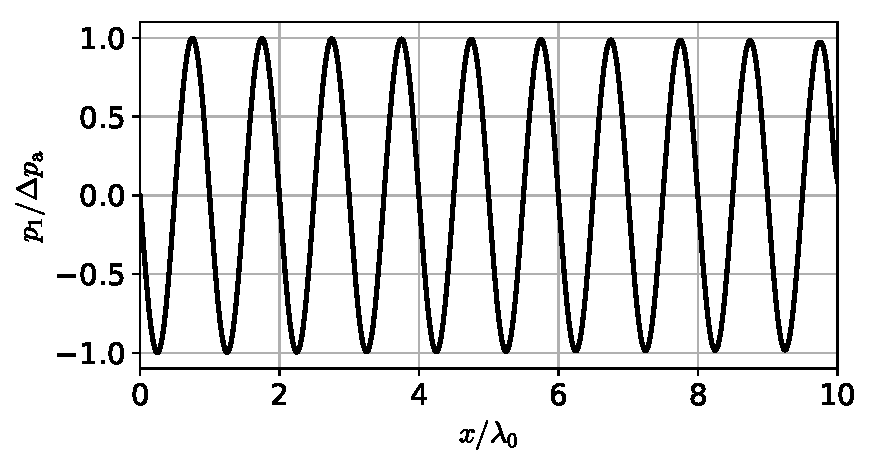
\includegraphics[width=0.5\textwidth]{DefaultRun.pdf}}
    \caption{\raggedright Instantaneous wave profile obtained for the default settings (empty {\tt run.DNA} file).}
    \label{fig:DefaultRun}
\end{figure}


\section{Absorbing vs reflecting boundary conditions}
\label{sec:Absorbing vs reflecting boundary conditions}

This example is found in {\tt examples/ScatteringAbsorbing}.

This test case illustrates the options for the boundary conditions. A Gaussian pulse is emitted as indicated by the red lines in Fig.~\ref{fig:BC} (see the {\tt run.DNA} file). The pulse is emitted at $x=0$ and travels from left to right. In Fig.~\ref{fig:BC} (a), the settings are:

{\tt
BoundaryConditionEast scattering\\
BoundaryConditionWest scattering
}

With the {\tt scattering} condition at the East boundary, the pulse is reflected at the boundary as indicated by the black line in Fig.~\ref{fig:BC} (a). In Fig.~\ref{fig:BC} (b), the settings are:

{\tt
BoundaryConditionEast absorbing\\
BoundaryConditionWest scattering
}

With the {\tt absorbing} condition at the East boundary, the pulse leaves the domain without reflection as shown by the black line in Fig.~\ref{fig:BC} (b). The settings for the West boundary are arbitrary as this boundary is the emission node in this case.

\begin{figure}
    \centering
    \subfloat[Scattering boundary]
    {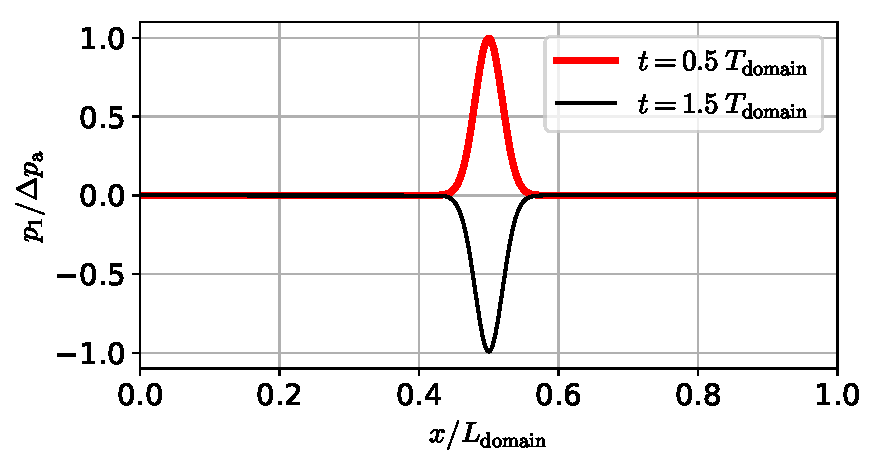
\includegraphics[width=0.49\textwidth]{px_scattering.pdf}} \
    \subfloat[Absorbing boundary]
    {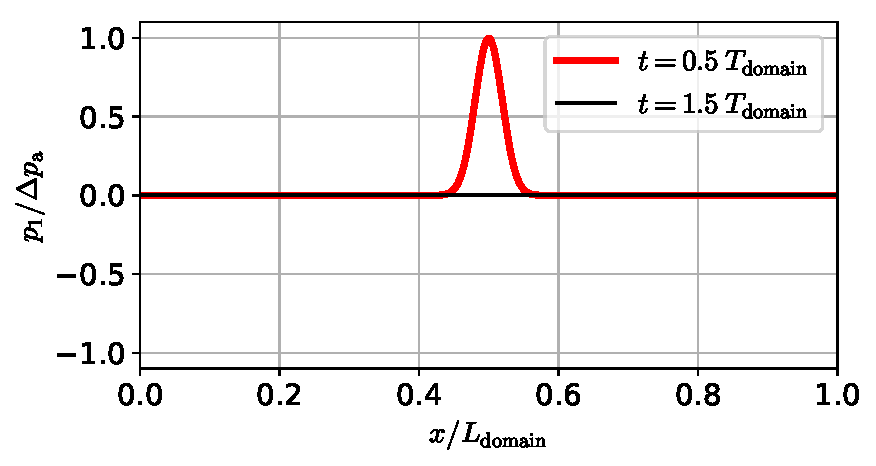
\includegraphics[width=0.49\textwidth]{px_absorbing.pdf}}
    \caption{\raggedright Illustration of the {\tt scattering} (b) and the {\tt absorbing} (b) boundary condition. A pulse travels from left to right (red lines). In (a), the pulse is reflected at the East domain boundary and travels back to the left (black line). In (b), the pulse passes the domain so that no reflection is visible (black line).}
    \label{fig:BC}
\end{figure}


\section{Shock-driven attenuation}
\label{sec:Shock-driven attenuation}

This example is found in {\tt examples/ShockDrivenAttenuation}.

This test case is concerned with the progressive deformation, shock formation, and shock-driven attenuation of an initially sinusoidal wave. The background medium is quiescent and the computational domain is at rest throughout the entire simulation. The $\mathrm{CFL}$ number is 0.05 with a spatial resolution of $N_{\mathrm{ppw}}=400$ points per wavelength $\lambda_0$ and a corrector weight of $\gamma=1.5$, set as follows:

{\tt
FluidNonLinearity 3.5
}

This rather high resolution is needed in order avoid excessive numerical dissipation due to the presence of the steep wavefront. The wave is emitted at the left boundary and travels to the right. The excitation amplitude and the nonlinearity coefficient $\beta$ are set in such a way that the nominal shock formation distance, given by \citep{Blackstock_1966}
\begin{equation}
    x_{\mathrm{sh}} = \dfrac{\rho_0 c_0^3}{2\pi \beta f_{\mathrm{a}}\Delta p_{\mathrm{a}}},
    \label{eq:xsh}
\end{equation}
takes the value $x_{\mathrm{sh}}=10$. At the shock formation distance, the progressively steepening wavefront first starts to develop a discontinuity. The red dashed line in Fig.~\ref{fig:shock_attenuation} represents the envelope $\widehat{p}_1$ owing to the Fay solution \citep{Fay_1931}, given by \citep{Blackstock_1966}
\begin{equation}
    \dfrac{\widehat{p}_1}{\Delta p_{\mathrm{a}}} = \dfrac{\pi}{1 + x/x_{\mathrm{sh}}}.
    \label{eq:Fay}
\end{equation}
The Fay solution is not applicable to the close vicinity of the emitter, but asymptotically approaches the wave profile decay at distances larger than approximately $3x_{\mathrm{sh}}$, where the initially sinusoidal has fully evolved into a saw-tooth shape. Fig.~\ref{fig:shock_attenuation} (a) shows that the wave profile exhibits only a minor decay prior to the shock formation distance, after which starts to approach the Fay envelope. Fig.~\ref{fig:shock_attenuation} (b) shows a detail of the fully developed saw-tooth pattern. It is noted that the predictor-corrector method drives the attenuation associated with the dissipation across the shock front. See \citet{Schenke_et_al_2022} for further discussions of this effect.

\begin{figure}
    \centering
    \subfloat[Decaying shock amplitude]
    {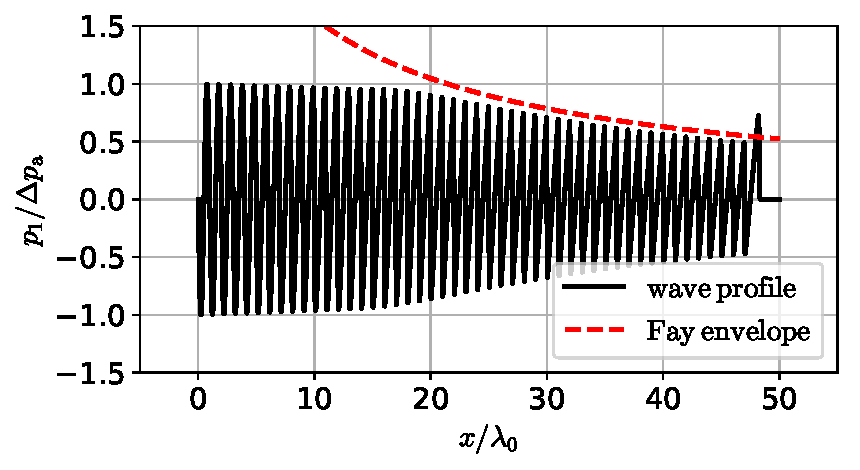
\includegraphics[width=0.49\textwidth]{shock_attenuation.pdf}}
    \subfloat[Detail of the saw-tooth profile]
    {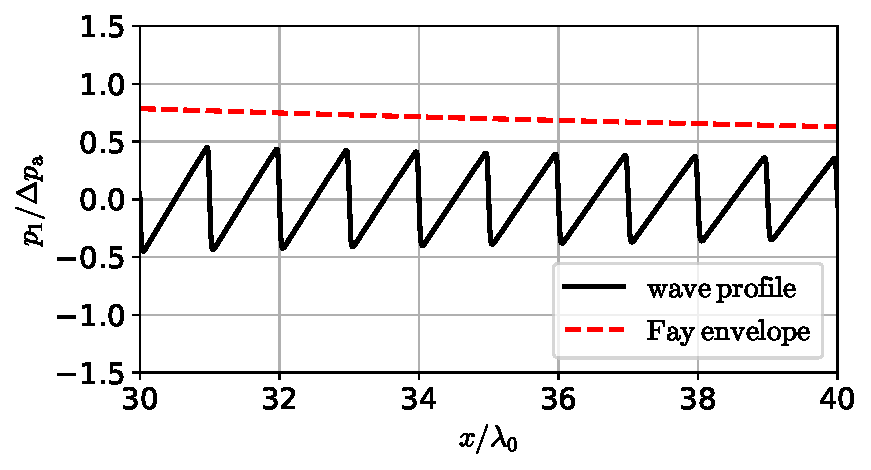
\includegraphics[width=0.49\textwidth]{shock_attenuation_detail.pdf}}
    \caption{\raggedright Initially sinusoidal and progressively steepening and shock-forming wave. As the wave has traveled past the shock formation distance $x_{\mathrm{sh}}=10\lambda_0$ (see Eq. \eqref{eq:xsh}) in subfigure (a), its amplitude starts to decay rapidly, asymptotically approaching the envelope of Fay solution \citep{Fay_1931} as given by Eq. \eqref{eq:Fay} \citep{Blackstock_1966}. Subfigure (b) depicts a detail of the fully developed saw-tooth profile.}
    \label{fig:shock_attenuation}
\end{figure}


\section{Moving emitter, boundary and flow}
\label{sec:Moving emitter, boundary and flow}

The following examples are found in {\tt examples/MovingBoundary}.

\subsection{Moving emitter}
\label{sec:Moving emitter}

This example is found in {\tt examples/MovingBoundary/RelativeEmitterMotion}.

This example illustrates how the Doppler shift due to the motion of an emitter relative to a quiescent medium can be reproduced with {\tt Wave-DNA}. A sine wave is excitated at the left (West) domain boundary and travels from left to right. The background flow field is quiescent:

{\tt BackgroundMotionMode quiescent}

The speed of sound is:

{\tt SoundSpeed 1500.0}

The moving boundary moves at a constant velocity magnitude of $500\:\mathrm{m/s}=c_0/3$, where the setting

    {\tt BoundaryMotionType linear}

is used to indicate a constant velocity of the boundary. The excitation location at the left boundary (default) is specified by:

{\tt ExcitationNode 0}

The initial position of the moving boundary is $x=0$ (default) and the fixed boundary is located at $x=0.18\:\mathrm{m}$ (12 times the unmodulted waveength $\lambda_0$), specified as follows:

{\tt
InitialMovingBoundaryPosition 0.0 \\
FixedBoundaryPosition 0.18
}

Hence, the moving boundary acts as a wave emitting boundary so that the acoustic wave is Doppler-shifted upon emission. In Fig.~\ref{fig:RelativeEmitterMotion} (a), the wave emitting boundary moves from right to left, hence against the direction of wave propagation, by setting:

{\tt MovingBoundaryVelocityAmplitude -500}

This causes a red-shift (frequency decrease) of the emitted wave. In Fig.~\ref{fig:RelativeEmitterMotion} (b), the wave emitting boundary moves from left to right, hence in the direction of wave propagation, by setting:

{\tt MovingBoundaryVelocityAmplitude 500}

This causes a blue-shift (frequency increase) of the emitted wave.

\begin{figure}
    \centering
    \subfloat[Red-shifted wave]
    {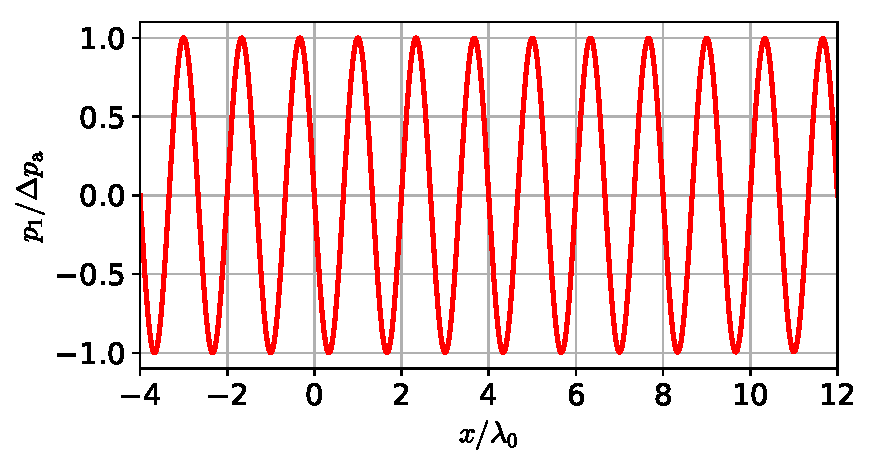
\includegraphics[width=0.49\textwidth]{Doppler_red.pdf}}
    \subfloat[Blue-shifted wave]
    {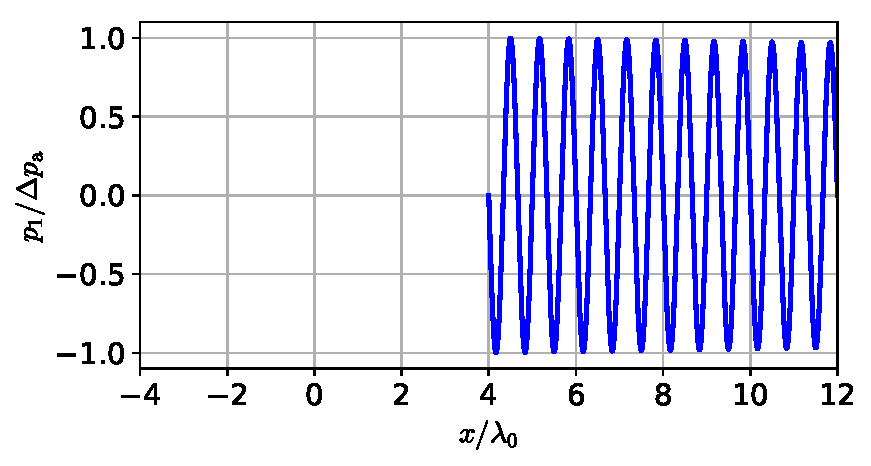
\includegraphics[width=0.49\textwidth]{Doppler_blue.pdf}}
    \caption{\raggedright Doppler-shift induced by an emitter moving relative to a quiescent medium: the wave is excited at the moving boundary. The wave emitting boundary starts at $x=0$ and moves in negative $x$-direction in (a), thereby red-shifting the emitted wave, and in positive $x$-direction in (b), thereby blue-shifting the emitted wave. The magnitude of the boundary velocity is $c_0/3$.}
    \label{fig:RelativeEmitterMotion}
\end{figure}


\subsection{Induced flow field}
\label{sec:Induced flow field}

This example is found in {\tt examples/MovingBoundary/InducedFlow}.

Fig.~\ref{fig:ConvectedWave} shows how an acoustic wave is Doppler-shifted by a temporaily constant and spatially uniform background flow field in one-dimensional Cartesian coordinates. In both Figs. \ref{fig:ConvectedWave} (a) and (b), the left domain boundary moves to the right with a velocity of $c_0/3$, and in both cases it induces a background flow field of the same velocity and direction by setting:

{\tt
BackgroundMotionMode coupledToMovingBoundary
}

In Fig.~\ref{fig:ConvectedWave} (a), the wave is excited at the moving boundary, which is initially at $x=0$ by setting:

{\tt
ExcitationNode 0
}

As a result, the wave travels from left to right and there is no relative motion between the wave emitter and the background flow field and the emitted wavelength $\lambda_0$ is not modulated. The instantaneous wave profile in Fig.~\ref{fig:ConvectedWave} is shown at two time instances in order to illustrate the variable position of the wave emitting boundary. In Fig.~\ref{fig:ConvectedWave} (b), the wave is excited at the fixed right boundary by setting:

{\tt
ExcitationNode 4800
}

Hence, the wave travels from right to left and the fixed wave emitting boundary is in relative motion to the encountered background flow field. This causes a blue-shift of the emitted wavelength.

\begin{figure}
    \centering
    \subfloat[Flow inducing and wave emitting boundary]
    {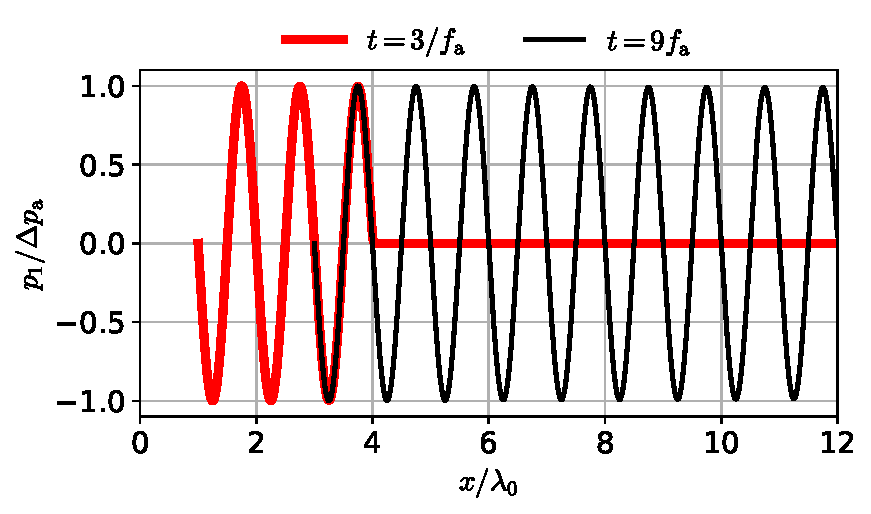
\includegraphics[width=0.49\textwidth]{InducedFlow.pdf}}
    \subfloat[Flow moving relative to fixed emitter]
    {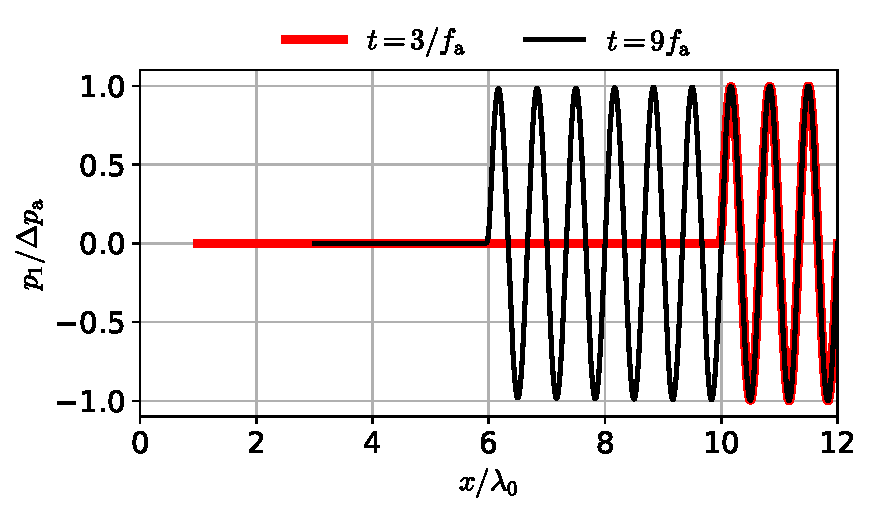
\includegraphics[width=0.49\textwidth]{RelativeEmitterMotion.pdf}}
    \caption{\raggedright Illustration of a flow-induced Doppler shift. The left domain boundary is initially at $x=0$ and moves from left to right with a velocity of $c_0/3$. At the same time, the moving boundary induces a temporarily and spatially constant background flow field. In (a), the wave is excited at the moving boundary and travels from left to right. As there is no relative motion between background medium in (a), the emitted wavelength is not modulated. In (b), the wave is excited at the right boundary and travels from right to left, so that the wave emitting boundary is in relative motion to the encountered background flow. This causes a blue-shift of the emitted wave.}
    \label{fig:ConvectedWave}
\end{figure}


\section{Possible combinations of moving boundaries, flow fields and emitters}
\label{sec:Possible combinations of moving boundaries, flow fields and emitters}

In {\tt examples/MovingBoundary/PossibleCombinations}, the possible combinations of setting up moving boundaries wave-emitting or non-emitting boundaries and quiescent or induced moving flow fields are demonstrated. Table \ref{tab:hierarchyMotion} illustrates the hierarchy of possible configurations.

The initial positions of the moving and the fixed boundary determines, which of them is identified as the West and the East boundary, where the boundary further to the left is the West boundary. The boundary condition (either {\tt scattering} or {\tt absorbing}) is assigned to the West and East boundaries, respectively ({\tt BoundaryConditionWest} or {\tt BoundaryConditionEast}). Irrespective of which of the two domain boundaries is the moving one, any of the two boundaries can be the wave-emitting boundary. It is recalled from Sec. \ref{sec:Wave excitation} that the wave-emitting boundary with instantaneous position $R\left(t\right)$ is alawys associated with grid node $0$, whereas the fixed boundary with position $R_{\mathrm{stat}}$ is always associated with grid node $N_{\mathrm{points}}-1$. Finally, for each of the four configurations of moving vs fixed and emitting vs non-emitting boundaries, the moving boundary can be a flow inducing one or move relative to a quiescent background flow field. This gives the eight different configurations as listed in Table \ref{tab:hierarchyMotion}.

Each of the test cases in this example directory is set up in such a way that waves move past the domain domain boundary. Hence, the test cases also illustrate how the wave-absorbing boundary condition is applied in these configurations.


\begin{table}[htb]
    \centering
    \begin{tabular}{|l|l|l|}
        \hline
        \multirow{4}{*}{Moving West boundary} & \multirow{2}{*}{Emitting West boundary ({\tt ExcitationNode} 0)}                       & Quiescent flow \\
        \cline{3-3}
                                              &                                                                                        & Induced flow   \\
        \cline{2-3}
                                              & \multirow{2}{*}{Emitting East boundary ({\tt ExcitationNode} $N_{\mathrm{points}}-1$)} & Quiescent flow \\
        \cline{3-3}
                                              &                                                                                        & Induced flow   \\
        \cline{1-3}
        \multirow{4}{*}{Moving East boundary} & \multirow{2}{*}{Emitting West boundary ({\tt ExcitationNode} $N_{\mathrm{points}}-1$)} & Quiescent flow \\
        \cline{3-3}
                                              &                                                                                        & Induced flow   \\
        \cline{2-3}
                                              & \multirow{2}{*}{Emitting East boundary ({\tt ExcitationNode} $0$)}                     & Quiescent flow \\
        \cline{3-3}
                                              &                                                                                        & Induced flow   \\
        \hline
    \end{tabular}
    \caption{Eight possible configurations of moving vs fixed, emitting vs non-emitting, and flow inducing vs relatively moving (quiescent flow) boundaries.}
    \label{tab:hierarchyMotion}
\end{table}


\section{Slowly oscillating emitter and flow field}
\label{sec:Slowly oscillating emitter and flow field}


The example of a slowly oscillating emitter is concerned with a slowly oscillating domain boundary, where ``slow'' means that the frequency $f_{\mathrm{b}}$ of the sinusoidal motion of the domain boundary is smaller than the emitted wave frequency $f_{\mathrm{a}}$. In this example, a spherically symmetric wave is considered, where the settings for the background flow field are:

{\tt
Geometry 3dSphericallySymmetric \\
BackgroundMotionMode quiescent \\
BackgroundVelocityScalingFactor 2.0
}

for a quiescent background medium to which the wave-emitting boundary is in relative motion or

    {\tt
        BackgroundMotionMode coupledToMovingBoundary\\
    }

for the case where the moving boundary displaces the fluid. The settings for the oscillatory boundary motion are:

{\tt
BoundaryMotionType oscillating \\
BoundaryMotionStartTime 0.0e-0 \\
BoundaryMotionEndTime 2.3e10 \\
InitialMovingBoundaryPosition 0.015 \\
FixedBoundaryPosition 0.195 \\
MovingBoundaryVelocityAmplitude 375 \\
MovingBoundaryFrequency 1e4
}

Hence, the boundary oscillates around an initial radius of $R_0=0.015\:\mathrm{m}$, which corresponds to one wavelength with an emitted wave frequency of $f_{\mathrm{a}}=100\:\mathrm{kHz}$ (ten times larger than the frequency the boundary motion) and a speed of sound of $c_0=1500\:\mathrm{m/s}$. With a velocity amplitude of $375\:\mathrm{m/s}$ of the boundary motion, the maximum Mach number is 0.25.

For reference, Fig.~\ref{fig:pr_oscilattingEmitter_staticBoundary} shows the instantaneous wave profile for a resting wave-emitting boundary ({\tt MovingBoundaryVelocityAmplitude 0}), where the wave decays like $1/r$ as indicated by the red dashed line. Figs. \ref{fig:rt_oscillatingEmitter} (a), (b), and (c) show the space-time diagrams for the resting, the relatively moving, and the flow-inducing moving boundaries, respectively. In the latter case, the characteristics posses a slight curvature due the variable background flow field in which the acoustic wave propagates.

\begin{figure}
    \centering
    {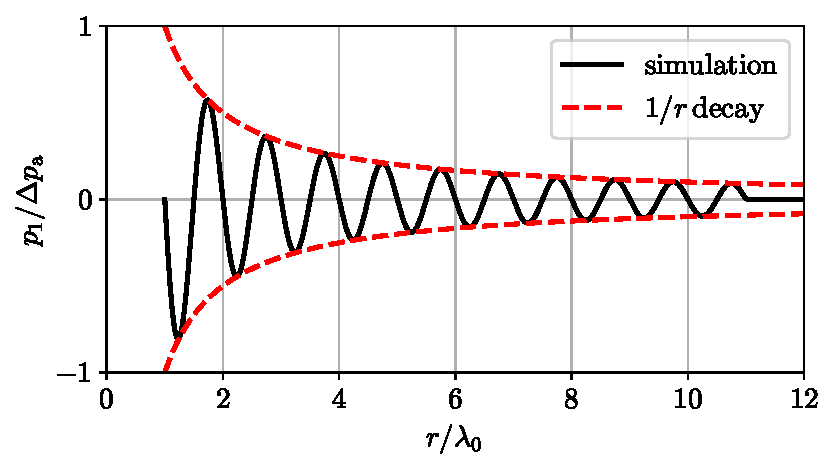
\includegraphics[width=0.5\textwidth]{pr_oscilattingEmitter_staticBoundary.pdf}}
    \caption{\raggedright spherically symmetric wave decaying like $1/r$.}
    \label{fig:pr_oscilattingEmitter_staticBoundary}
\end{figure}

\begin{figure*}
    %\baselineskip=12pt
    \subfloat[Fixed wave-emitting boundary]
    {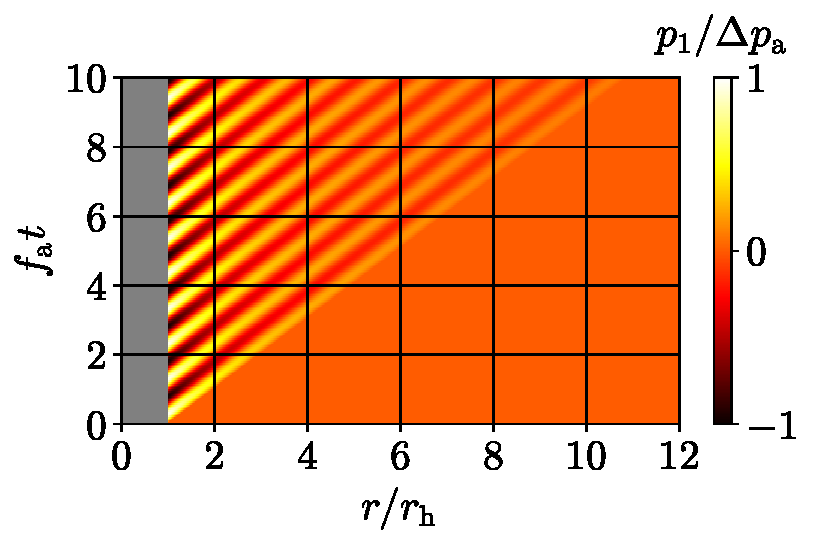
\includegraphics[width=0.33\textwidth]{rt_oscilattingEmitter_staticBoundary.pdf}}
    \subfloat[Oscillating wave-emitting boundary in a quiescent medium]
    {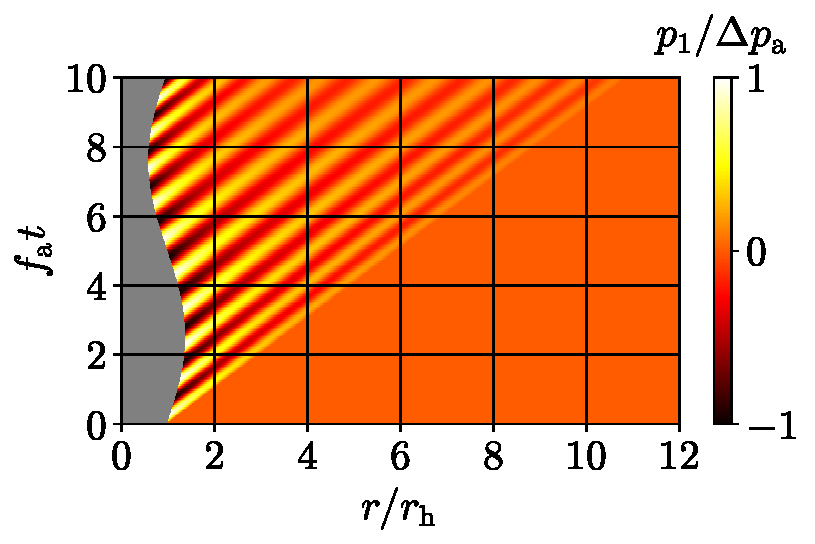
\includegraphics[width=0.33\textwidth]{rt_oscilattingEmitter_quiescent.pdf}}
    \subfloat[Oscillating flow-inducing wave-emitting boundary]
    {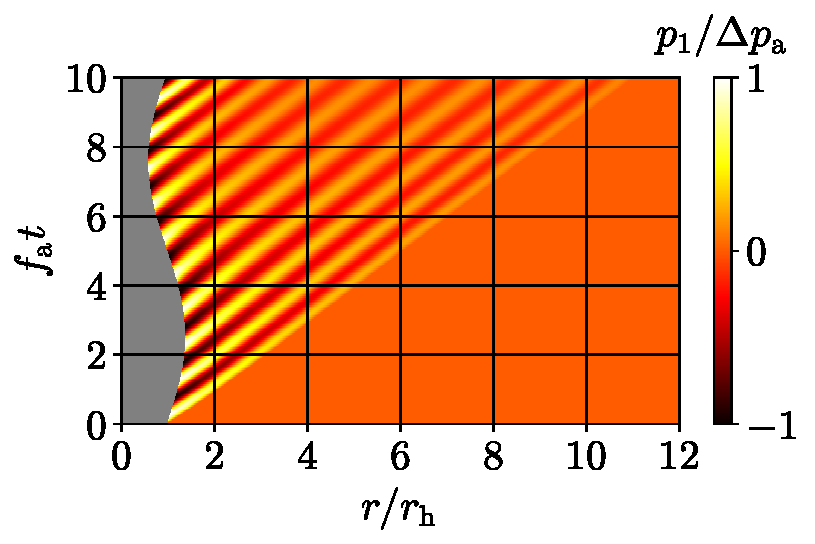
\includegraphics[width=0.33\textwidth]{rt_oscilattingEmitter_inducedFlow.pdf}}
    \caption{\raggedright Space-time diagrams of an oscillating wave-emitting boundary, where ten acoustic wave periods are emitted during one oscillation cycle of the moving boundary.}
    \label{fig:rt_oscillatingEmitter}
    %\vskip1in
\end{figure*}


\section{Acoustic black and white holes}
\label{sec:Acoustic black and white holes}

The following examples show how {\tt Wave-DNA} can be used to simulate the acoustic wave propgation in acoustic black and white hole configurations \citep{Schenke_et_al_2022_PoF}. The individual test case folders, containing illustrative acoustic black and white hole examples, include python postprocessing scripts in order to produce space-time diagrams, the plots of the instantaneous wave profiles, and the acoustic pressure evolution at the sonic horizon.

It is important to note that rather than representing compressible background flow fields with variable $\rho_0$ and $c_0$, the acoustic black/white hole configurations are model systems for acoustic waves propagating in accelerating flow fields of any (also subsonic) velocity magnitude. The reason for the acoustic black/white hole being such a convenient system for the computational study of acoustic waves in accelerating flow fields lies in the fact that they allow to trap a wave characteristic at the point of sonic transition, the sonic horizon, where it is subject to both a constant background flow velocity and a constant background flow acceleration. Due to the non-zero acceleration, the neighbouring characteristics are either converging towards or diverging away from the sonic horizon.

In the acoustic black hole example shown here, nonlinearities are neglected ($\beta=0$ and $\mathcal{L}=0$). Fig.~\ref{fig:BH} exemplarily shows (a) the space-time diagram and (b) the instantaneous acoustic pressure profiles for an acoustic black hole. The entire physical domain in Fig.~\ref{fig:BH} is initially located outside the acoustic black hole. Subsequently, the moving wave emitting boundary collapses and eventually passes the sonic horizon while emitting outgoing characteristics. The example in Fig.~\ref{fig:BH} is realized by the following boundary settings:

{\tt
BoundaryMotionType stationaryBlackHole \\
InitialMovingBoundaryPosition 1.60175 \\
FixedBoundaryPosition 1.75175
}

The stationary sonic horizon radius and the geometry settings are:

{\tt
Geometry 3dSphericallySymmetric \\
BackgroundMotionMode coupledToMovingBoundary \\
HorizonRadius 1.5
}

With these settings, the wave emitting boundary radiates a wavetrain that propagates in positive $r$-direction. At the same time, the spherical moving boundary collapses and induces an inward-directed spherically symmetric background fluid flow that satisfies Eq. \eqref{eq:u0_spherical}. The boundary satisfies Eq. \eqref{eq:R} so that a stationary flow field is obtained. The data at the stationary sonic horizon is written to the output file {\tt horizon.dat}. This file can be consulted to examine the evolution of the acoustic pressure and the acoustic (velocity) potential at the sonic horizon.

Fig.~\ref{fig:WH} exemplarily shows (a) the space-time diagram and (b) the instantaneous acoustic pressure profiles for an acoustic white hole, which can be seen as the inverse problem of the acoustic black hole. This time, the entire physical domain is initially located inside the acoustic white hole. Subsequently, the wave emitting boundary expands and eventually passes the sonic horizon while emitting ingoing characteristics. The sonic horizon radius, the speed of sound, and the emitted wave frequency are the same as in Fig.~\ref{fig:BH}. The settings to trap the same emitted wave period at the sonic horizon as in the acoustic black hole configuration are as follows:

{\tt
BOUNDARYMOTION \\
BoundaryMotionType stationaryWhiteHole \\
InitialMovingBoundaryPosition 1.3824 \\
FixedBoundaryPosition 1.2359
}

Furthermore, Fig.~\ref{fig:WH} shows the results for the nonlinear wave, which exhibits the well-known nonlinear wave-steepening. The settings to achieve the nonlinear wave propagation behavior, in this particular case dominated by the constitutive nonlinearity represented by the nonlinearity coefficient $\beta$ ({\tt FluidNonLinearity}), are:

    {\tt
        FluidNonLinearity 3.5 \\
        LocalNonlinearity True
    }

In the acoustic white hole in Fig.~\ref{fig:WH}, the characteristics converge towards the sonic horizon so that the acoustic wave is progressively blue-shifted while the acoustic wave amplitude increases over time.

\begin{figure*}
    %\baselineskip=12pt
    \subfloat[Space-time diagram]
    {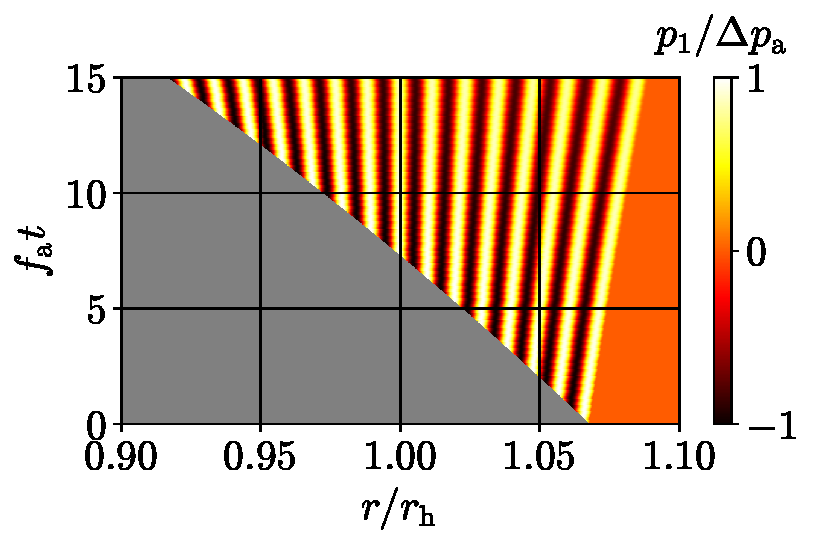
\includegraphics[width=0.45\textwidth]{rt_smallABH.pdf}}
    \subfloat[Instantaneous acoustic pressure profile]
    {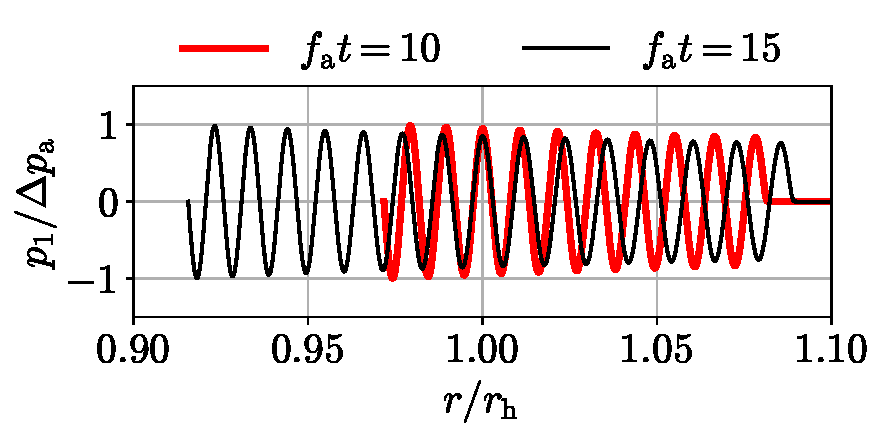
\includegraphics[width=0.45\textwidth]{pr_smallABH.pdf}}
    \caption{Example of an acoustic black hole.}
    \label{fig:BH}
    %\vskip1in
\end{figure*}


\begin{figure*}
    %\baselineskip=12pt
    \subfloat[Space-time diagram]
    {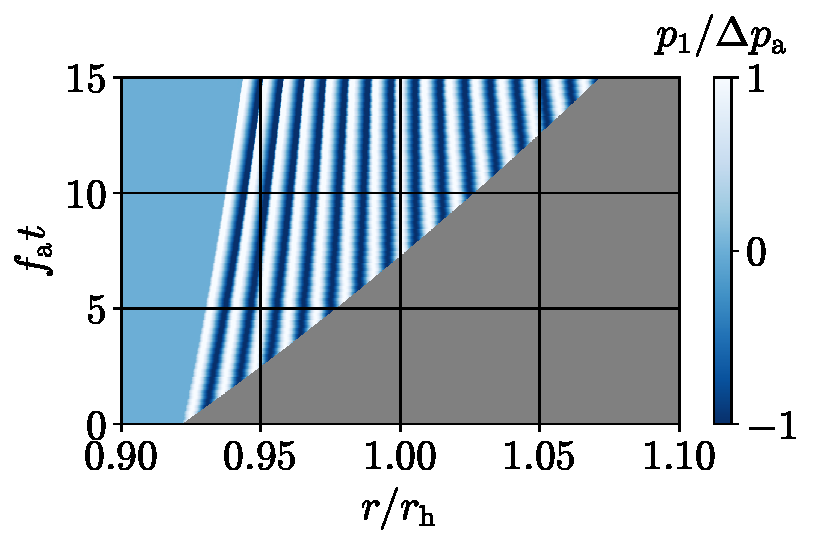
\includegraphics[width=0.45\textwidth]{rt_smallAWH_nonlin.pdf}}
    \subfloat[Instantaneous acoustic pressure profile]
    {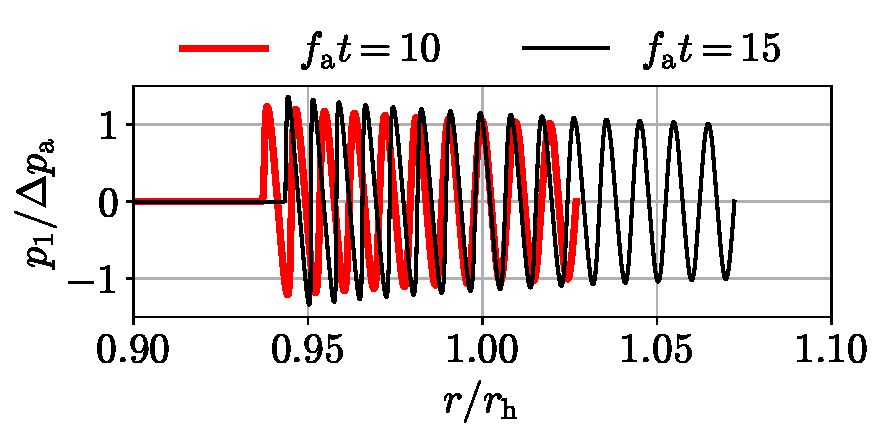
\includegraphics[width=0.45\textwidth]{pr_smallAWH_nonlin.pdf}}
    \caption{Example of an acoustic white hole.}
    \label{fig:WH}
    %\vskip1in
\end{figure*}




\chapter{Appendix}
\label{chap:Appendix}

Due to the rather large number of terms in the transformed wave equation, it is advantageous to derive it in two steps, leading to a hierarchy of coefficients. By first expanding the material derivatives in Eq. \eqref{eq:convectiveKuznetsov}, one gets
\begin{equation}
\mathcal{A}_1 \dfrac{\partial \phi_1}{\partial t}
+ \mathcal{A}_2 \dfrac{\partial^2 \phi_1}{\partial t^2}
+ \mathcal{K} \dfrac{\partial \phi_1}{\partial t}\dfrac{\partial^2 \phi_1}{\partial t^2}
+ \mathcal{A}_G \dfrac{\partial \phi_1}{\partial r} - \dfrac{c_0^2}{A}\dfrac{\partial A}{\partial r} \dfrac{\partial \phi_1}{\partial r} + \mathcal{A}_L \dfrac{\partial^2 \phi_1}{\partial r^2}
+ \mathcal{U} = 0,
\label{eq:convectiveKuznetsov_AAA}
\end{equation}
where the coefficients in Eq. \eqref{eq:convectiveKuznetsov_AAA} are given by
\begin{align}
& \mathcal{A}_1 = \mathcal{K}\left(\mathcal{U} + u_0^2\dfrac{\partial^2\phi_1}{\partial r^2}\right),
\label{eq:A1} \\
& \mathcal{A}_2 = 1 + \mathcal{K}u_0\dfrac{\partial \phi_1}{\partial r},
\label{eq:A2} \\
& \mathcal{A}_G = \dfrac{\partial u_0}{\partial r}\dfrac{\partial \phi_1}{\partial r} + 2\dfrac{\partial^2 \phi_1}{\partial r\partial t} + \mathcal{K}u_0 \mathcal{U},
\label{eq:AG} \\
& \mathcal{A}_L = u_0^2 - c_0^2 + 2u_0\dfrac{\partial \phi_1}{\partial r} + \mathcal{K}u_0^3\dfrac{\partial \phi_1}{\partial r},
\label{eq:AL}
\end{align}
and where
\begin{equation}
\mathcal{K} = \dfrac{2\left(\beta - 1\right)}{c_0^2},
\label{eq:Kcoeff}
\end{equation}
and
\begin{equation}
\mathcal{U} = 2u_0\dfrac{\partial^2 \phi_1}{\partial x\partial t} + \dfrac{\mathrm{D}u_0}{\mathrm{D}t}\dfrac{\partial\phi_1}{\partial r}.
\label{eq:Uterm}
\end{equation}
are recurring auxiliary variables. Following \citet{Solovchuk_et_al_2013}, the nonlinear term in Eq. \eqref{eq:convectiveKuznetsov_AAA} is linearized by applying the Newton linearization
\begin{equation}
\dfrac{\partial \phi_1}{\partial t}\dfrac{\partial^2 \phi_1}{\partial t^2} \approx
\left(\dfrac{\partial \phi_1}{\partial t}\right)^o\dfrac{\partial^2 \phi_1}{\partial t^2}
+
\left(\dfrac{\partial^2 \phi_1}{\partial t^2}\right)^o\dfrac{\partial \phi_1}{\partial t}
- \left(\dfrac{\partial \phi_1}{\partial t}\right)^o\left(\dfrac{\partial^2 \phi_1}{\partial t^2}\right)^o.
\label{eq:NewtonLin}
\end{equation}
In a second step, Eqs. \eqref{eq:transDerivativeOp_space} and \eqref{eq:transDerivativeOp_time} are applied to Eq. \eqref{eq:convectiveKuznetsov_AAA} in order to change the variables from $r$ to $\xi$. This results in the transformed wave equation
\begin{equation}
\mathcal{B}_1 \dfrac{\partial \Phi_1}{\partial t}
+ \mathcal{B}_2 \dfrac{\partial^2 \Phi_1}{\partial t^2}
+ 2\mathcal{B}_2 \dfrac{\partial \xi}{\partial t} \dfrac{\partial^2 \Phi_1}{\partial \xi\partial t}
+ \mathcal{B}_G \dfrac{\partial \Phi_1}{\partial \xi}
+ \mathcal{B}_L \dfrac{\partial^2 \Phi_1}{\partial \xi^2}
- \dfrac{c_0^2}{A}\dfrac{\partial A}{\partial r} \dfrac{\partial \xi}{\partial r}\dfrac{\partial \Phi_1}{\partial \xi}
+ \mathcal{U}
- \mathcal{K}\left(\dfrac{\partial \phi_1}{\partial t}\right)^o\left(\dfrac{\partial^2 \phi_1}{\partial t^2}\right)^o
= 0
\label{eq:convectiveKuznetsov_BBB}
\end{equation}
with the coefficients
\begin{align}
& \mathcal{B}_1 = \mathcal{A}_1 + \mathcal{K}\left(\dfrac{\partial^2 \phi_1}{\partial t^2}\right)^o,
\label{eq:B1} \\
& \mathcal{B}_2 = \mathcal{A}_2 + \mathcal{K}\left(\dfrac{\partial \phi_1}{\partial t}\right)^o,
\label{eq:B2} \\
& \mathcal{B}_G =
\mathcal{B}_1\dfrac{\partial \xi}{\partial t}
+ \mathcal{B}_2\left(\dfrac{\partial^2\xi}{\partial t^2} + \dfrac{\partial \xi}{\partial t} \dfrac{\partial^2\xi}{\partial t\partial \xi}\right)
+ \dfrac{\partial \xi}{\partial r}\left(\mathcal{A}_G
+ \mathcal{A}_L\dfrac{\partial^2\xi}{\partial r\partial \xi}\right),
\label{eq:BG} \\
& \mathcal{B}_L = \mathcal{B}_2\left(\dfrac{\partial \xi}{\partial t}\right)^2 + \mathcal{A}_L\left(\dfrac{\partial \xi}{\partial r}\right)^2,
\label{eq:BL}
\end{align}
which again depend on the coefficients $\mathcal{A}_{...}$ given by Eqs. \eqref{eq:A1} to \eqref{eq:AL} derived in the previous step. In the present numerical framework, the mixed spatial-temporal derivative in Eq. \eqref{eq:convectiveKuznetsov_BBB} is treated fully explicitly. However, it turns out be beneficial regarding the numerical accuracy to substitute the term by the following equivalent expression prior to the discretization. The equivalent expression is obtained by expanding $\partial^2\left(\Phi_1\partial\xi/\partial t\right)/\partial \xi \partial t$, resulting in
\begin{equation}
\dfrac{\partial \xi}{\partial t} \dfrac{\partial^2 \Phi_1}{\partial \xi\partial t}
= \dfrac{1}{2}\dfrac{\partial \xi}{\partial t} \dfrac{\partial^2 \Phi_1}{\partial \xi\partial t} +
\dfrac{1}{2}\left[
\dfrac{\partial^2}{\partial \xi\partial t}\left(\dfrac{\partial \xi}{\partial t}\Phi_1\right)
- \dfrac{\partial^2 \xi}{\partial t^2 \partial \xi} \dfrac{\partial \Phi_1}{\partial \xi}
- \dfrac{\partial^3 \xi}{\partial t^2\partial \xi}\Phi_1
- \dfrac{\partial^2 \xi}{\partial t \partial \xi} \dfrac{\partial \Phi_1}{\partial t}\right].
\label{eq:mixedTerm}
\end{equation}


\cleardoublepage

\addcontentsline{toc}{chapter}{Bibliography}
\bibliographystyle{plainnat}
%\bibliography{/Users/fabian/Zotero/library}
\bibliography{library}
\end{document}
